\BourbakiExercises{习题}

\begin{enumerate}
\def\labelenumi{\arabic{enumi})}
\tightlist
\item
  设 D 是一个体，V 是 D 上的一个右向量空间，A 是环 \(\operatorname{End}_{\mathbb{D}}(\mathrm{V})\)。对 V 的任一线性子空间 W，用 \(\mathfrak{a}(\mathrm{W})\)（相应地，b(W)）表示 A 中满足 aW = 0（相应地，aV ⊂ W）的元素 a 所成的集。
\end{enumerate}

\begin{enumerate}
\def\labelenumi{\alph{enumi})}
\item
  证明映射 \(W \mapsto \mathfrak{a}(W)\)（相应地，\(W \mapsto \mathfrak{b}(W)\)）是从 V 的线性子空间之集到 A 的由幂等元生成的左（相应地，右）理想之集上的一个递减（相应地，递增）双射。
\item
  A 的极小左理想是诸理想 \(\mathfrak{a}(\mathrm{H})\)，其中 H 是 V 中一个超平面。A 的极小右理想是诸理想 \(\mathfrak{b}(\mathrm{D})\)，其中 D 是 V 中一条直线。由此推出 A 的有限长度的左（相应地，右）理想的形式。
\item
  设 W 与 \(W'\) 是 V 的两个子空间，满足 \(W \neq 0\) 且 \(W' \neq V\)。证明交 \(\mathfrak{a}(W) \cap \mathfrak{b}(W')\) 不约化为 0。
\end{enumerate}

\(d\) ) 映射 \(u\mapsto{}^{t}u\) 定义了从 A 到 \(\mathrm{End}_{\mathrm{D}^{\circ}}(\mathrm{V}^{*})\) 的一个子环 B 的环同构。证明在此同构下，\(\mathfrak{a}(\mathrm{W})\)（相应地，\(\mathfrak{b}(\mathrm{W}))\)）的像是理想 \(\mathfrak{b}(\mathrm{W}^{\circ})\)（相应地，\(\mathfrak{a}(\mathrm{W}^{\circ}))\)）在 B 上的迹，其中 \(\mathrm{W}^{\circ}\) 表示 W 在 \(\mathrm{V}^*\) 中的正交

\begin{enumerate}
\def\labelenumi{\alph{enumi})}
\setcounter{enumi}{4}
\tightlist
\item
  设 \(\mathfrak{F}\) 是 V 的线性子空间所成的集。对 A 的任一左理想 \(\mathfrak{a}\)，用 \(\mathfrak{F}(\mathfrak{a})\) 表示 \(\mathfrak{F}\) 中由诸子空间 \(\operatorname{Ker} u\)（\(u\) 取遍 \(\mathfrak{a}\)）组成的子集。集 \(\mathfrak{F}(\mathfrak{a})\) 对交运算稳定，且 V 的每个包含 \(\mathfrak{F}(\mathfrak{a})\) 中一个元素的线性子空间都属于 \(\mathfrak{F}(\mathfrak{a})\)。证明映射 \(\mathfrak{a} \mapsto \mathfrak{F}(\mathfrak{a})\) 是从 A 的左理想之集到 \(\mathfrak{F}\) 的具有这两条性质的子集之集上的一个双射。f) 设 V 的维数无限，并用 \(\mathfrak{c}\) 表示它。设 \(\mathfrak{m}\) 是 A 的一个极大左理想，它不具有 \(\mathfrak{a}(D)\) 的形式。证明诸子空间 \(W \in \mathfrak{F}(\mathfrak{m})\) 的交约化为 0，这些子空间中的每一个都是无限维的，并且存在余维数为 \(\mathfrak{c}\) 的这样的子空间。
\end{enumerate}

¶ 2) 设 D 是一个体，V 是 D 上一个无限维 c 的右向量空间，A 是环 \(\operatorname{End}_{\mathbb{D}}(\mathbb{V})\)。

\begin{enumerate}
\def\labelenumi{\alph{enumi})}
\item
  设 u 与 v 是 V 的自同态，满足 \(\operatorname{rg}(u) \leqslant \operatorname{rg}(v)\)。证明存在 A 的元素 a 与 b，使得 u = avb。
\item
  对任一无限基数 \(n \leqslant c\)，把 V 的秩 \textless{} n 的自同态所成的集记作 \(A_{n}\)。证明 \(A_{n}\) 是 A 的一个双边理想，并且 A 的每个异于 \(\{0\}\) 与 A 的双边理想都是某个 \(A_{n}\)（利用 a)）。特别地，有限秩自同态的理想是 A 的最小非零双边理想，而理想 \(A_{c} = T\)（由秩 \textless{} c 的自同态组成）是 A 的异于 A 的最大双边理想。
\item
  设 B 是 V 的一个基，U 是 B 上的一个超滤子，它比由 B 的基数 \textless{} c 的子集的补集组成的滤子 G 更细。对 U 中每个集 U，用 \(e_{U}\) 表示 V 的投影算子，其核由 U 的向量生成，其像由 B-U 的向量生成。用 \(a_{U}\) 表示由诸 \(e_{U}\)（其中 U 取遍 U）生成的 A 的左理想。证明理想 \(T + a_{U}\) 异于 A。设 V 是 B 上另一个包含 G 且异于 U 的超滤子。证明我们有 \(a_{U} + a_{V} = A\)。d) 证明 B 上包含 G 的超滤子所成的集的基数是 \(2^{2^{c}}\)。（利用一般拓扑，I, §8, 第 135 页习题 6 与一般拓扑，I, §4, 第 126 页习题 5 的论证。注意在后一习题中，X 的每个非空开子集在 F 上的迹与 F 具有相同的基数。）
\item
  设 \(\operatorname{Card}(\mathrm{D}) \leqslant 2^{\mathfrak{c}}\)。由 \(d\) 推出，单 \((\mathrm{A} / \mathfrak{T})\)-模的类所成的集具有基数 \(2^{2^{\mathfrak{c}}}\)（参见 VIII, 第 52 页，习题 5, \(d\) )）。
\end{enumerate}

\(f\) ) 由上述推出，环 A 是本原的但不是拟单的，而环 \(\mathrm{A} / \mathfrak{T}\) 是拟单的但不是单的（VIII, 第 120 页，注 2）。

\begin{enumerate}
\def\labelenumi{\arabic{enumi})}
\setcounter{enumi}{2}
\tightlist
\item
  设 \(D\) 是一个体，\(V\) 是 \(D\) 上的一个右向量空间，\(A\) 是环 \(\operatorname{End}_D(V)\) 的一个子环。
\end{enumerate}

\begin{enumerate}
\def\labelenumi{\alph{enumi})}
\tightlist
\item
  证明下列条件等价：
\end{enumerate}

\begin{enumerate}
\def\labelenumi{(\roman{enumi})}
\item
  对每个自同态 \(u\)（\(V\) 的）与向量的每个有限序列 \(x_{1},\ldots ,x_{n}\)（在 \(V\) 中），存在一个元素 \(a\)（\(A\) 的），满足 \(u(x_{i}) = a(x_{i})\)（对 \(1\leqslant i\leqslant n\)）。
\item
  对每对元素 \(x, y\)（\(V\) 的，\(x \neq 0\)），存在 \(a \in A\)，使得 \(a(x) = y\)。
\end{enumerate}

当这些条件满足时，我们称 \(\operatorname{End}_{\mathbb{D}}(\mathrm{V})\) 的子环 A 是稠密的。从现在起设 A 是稠密的。

\begin{enumerate}
\def\labelenumi{\alph{enumi})}
\setcounter{enumi}{1}
\item
  证明 A 是本原的（VIII, 第 120 页，注 2）。反之，证明每个本原环都同构于某个向量空间的自同态环的一个稠密子环。
\item
  证明 A 的中心的非零元素都是单自同态。特别地，本原环的中心是一个整环。
\item
  设 V 是无限维的。对每个整数 n \textgreater{} 0，证明存在 A 的一个子环 \(A_{n}\) 和一个满同态 \(\mathrm{A}_{n} \to \mathbf{M}_{n}(\mathrm{D})\)。
\end{enumerate}

\begin{enumerate}
\def\labelenumi{\arabic{enumi})}
\setcounter{enumi}{3}
\tightlist
\item
  设 \(\mathrm{A}\) 是一个本原环。
\end{enumerate}

\begin{enumerate}
\def\labelenumi{\alph{enumi})}
\item
  若环 A 是交换的（相应地，左阿廷的），则它是一个体（相应地，一个单环）。
\item
  设 a 与 b 是 A 的非零左理想。证明理想 ab 不为零。\(^{(3)}\) 由此推出 A 的有限多个非零双边理想的交不约化为 0。

  \( ^{(3)} \) 在本习题与下一习题中，若 a 与 b 是 A 的左理想，则用 ab 表示由诸乘积 ab（\(a \in a\)，\(b \in b\)）生成的左理想。
\item
  证明若对每个 \(a \in A\)，元素 \(1 + a^{2}\) 在 A 中可逆，则 A 是一个体（利用习题 3, b)）。
\end{enumerate}

\begin{enumerate}
\def\labelenumi{\arabic{enumi})}
\setcounter{enumi}{4}
\tightlist
\item
  设 \(\mathrm{A}\) 是一个环。
\end{enumerate}

\begin{enumerate}
\def\labelenumi{\alph{enumi})}
\item
  设 e 是 A 中的幂等元。证明若 A 是本原的（相应地，拟单的），则环 eAe 亦然（利用习题 3, b)，VIII, 第 113 页的引理 4，以及 VIII, 第 15 页的习题 6, a)）。
\item
  设 n 是一个整数 \(\geqslant 1\)。证明矩阵环 \(\mathbf{M}_{n}(\mathrm{A})\) 是本原的（相应地，拟单的）当且仅当 A 是本原的（相应地，拟单的）（参见 VIII, 第 114 页，例 2）。
\item
  设 B 是一个与 A 森田等价的环；则 B 是本原的（相应地，拟单的）当且仅当 A 亦然。
\end{enumerate}

\begin{enumerate}
\def\labelenumi{\arabic{enumi})}
\setcounter{enumi}{5}
\tightlist
\item
  设 \(A\) 是一个拟单环。
\end{enumerate}

\begin{enumerate}
\def\labelenumi{\alph{enumi})}
\item
  一个 A-模是生成模当且仅当它的对偶非零。
\item
  设 \(\mathfrak{a}\) 是 A 的一个左理想，D 是环 \(\operatorname{End}_{\mathrm{A}}(\mathfrak{a})\)。证明 \(\mathfrak{a}\) 是一个有限生成的投射右 D-模，且映射 \(a \mapsto a_{\mathfrak{a}}\)（从 A 到 \(\operatorname{End}_{\mathrm{D}}(\mathfrak{a})\)）是双射。环 D 是拟单的当且仅当 A-模 \(\mathfrak{a}\) 是投射的且有限生成的。
\item
  证明一个包含极小左理想的拟单环是单的。
\end{enumerate}

\begin{enumerate}
\def\labelenumi{\arabic{enumi})}
\setcounter{enumi}{6}
\tightlist
\item
  设 A 是一个环。
\end{enumerate}

\begin{enumerate}
\def\labelenumi{\alph{enumi})}
\item
  设 \(\mathfrak{a}\) 是 A 的一个极小左理想。证明我们有 \(\mathfrak{a}^2 = 0\) 或 \(\mathfrak{a}^2 = \mathfrak{a}\)。在后一情形，证明存在一个幂等元 \(e\)（在 \(\mathfrak{a}\) 中），使得 \(\mathfrak{a} = \mathrm{A}e\)（若 \(a \in \mathrm{A}\) 满足 \(\mathfrak{a}a = \mathfrak{a}\)，考虑自同构 \(x \mapsto xa\)（\(\mathfrak{a}\) 的））。
\item
  设 e 是 A 中的幂等元。理想 Ae 是极小的当且仅当环 eAe 是一个体。
\item
  设 \(\mathfrak{a}\) 与 \(\mathfrak{b}\) 是 A 的两个同构的左理想。证明我们有 \(\mathfrak{ab} = \mathfrak{b}\)（若 \(\mathfrak{a}^2 = \mathfrak{a}\)），而 \(\mathfrak{ab} = 0\)（若 \(\mathfrak{a}^2 = 0\)）。
\end{enumerate}

¶ 8) 设 A 是一个环。A 的左底座（或简称底座）s 是 A-模 \(A_{s}\) 的底座，即（VIII, 第 65 页）A 的极小左理想之和。它是一个半单 A-模，而它的同型分量称为它的足。设 a 是 s 的一个足。

\begin{enumerate}
\def\labelenumi{\alph{enumi})}
\item
  证明 \(\mathfrak{a}\) 是一个双边理想，并且含于 \(\mathfrak{a}\) 的诸平方为零的极小理想（习题 7）之和是一个双边理想，即 \(\mathfrak{a}\) 与其零化子之交。
\item
  设 a 包含一个平方非零的极小理想。证明不存在 a 的非零元素 x 满足 ax = 0（利用习题 7, c)）。
\item
  在 b) 的假设下，证明伪环 a（I, §8, No.~1, 第 98 页）的每个左理想都是 A 的理想（注意 a 的极小理想就是 A 的含于 a 的极小理想）。
\item
  设 A 的底座 s 不包含任何平方为零的极小左理想。证明 A 的每个作为 A-模具有有限长度的左理想 b 都含于 \(\mathfrak{s}\)（对 \(\mathfrak{b}\) 的长度用归纳法，注意若 \(e\) 是 \(\mathfrak{b}\) 中的幂等元，则 \(\mathfrak{be}\) 是 \(\mathfrak{b}\) 的一个直因子）。
\end{enumerate}

¶ 9) 设 D 是一个体，V 是 D 上的一个右向量空间，A 是环 \(\operatorname{End}_{\mathrm{D}}(\mathrm{V})\) 的一个稠密子环（习题 3）。

\begin{enumerate}
\def\labelenumi{\alph{enumi})}
\item
  子环 A 包含一个非零的有限秩自同态，当且仅当 A 的底座 s 非零（利用习题 4, a) 与 7, b) 证明 A 的极小理想由一个幂等元生成，再证明该幂等元的秩为 1）。此时 A 的底座只有单个足（习题 4, a)）。
\item
  从现在起设 \(s \neq 0\)。设 a 是 A 的一个极小左理想。证明存在一个元素 \(\ell\)（V 的对偶 \(V^{*}\) 的），使得 a 由诸自同态 \(z \mapsto v \ell(z)\)（\(v \in V\)）组成。设 \(V'\) 是由线性型 \(\ell \in V^{*}\) 组成的集，这些线性型使得自同态 \(z \mapsto v \ell(z)\) 对每个 \(v \in V\) 都属于 A。证明 \(V'\) 是 \(V^{*}\) 的一个 (D, A)-子双模，且 s 是 V 的这样的有限秩自同态组成的集：其核可写成 \(\operatorname{Ker} \ell_{1} \cap \cdots \cap \operatorname{Ker} \ell_{n}\)，其中 \(\ell_{1}, \ldots, \ell_{n}\) 属于 \(V'\)。仅当向量空间 V 是有限维且 \(A = \operatorname{End}_{\mathrm{D}}(\mathrm{V})\) 时，才能有 s = A。
\item
  设 \(\mathfrak{b}\) 是 A 的一个极小右理想。证明存在向量 \(v \in V\)，使得 \(\mathfrak{b}\) 由诸自同态 \(z \mapsto v\ell(z)\)（\(\ell \in V'\)）组成。由此推出 A 的右底座等于其左底座 \(\mathfrak{s}\)。
\end{enumerate}

\(d\) ) 证明 \(\mathfrak{s}\) 还是 A 的最小非零双边理想。

\begin{enumerate}
\def\labelenumi{\alph{enumi})}
\setcounter{enumi}{4}
\tightlist
\item
  由 b) 推出，一个具有非零底座的（左或右）诺特本原环是单的（通过考虑含于 s 中的理想证明 V 必为有限维）。
\end{enumerate}

\(f\) ) 设 M 是 V 的一个有限维子空间。证明 \(\mathfrak{s}\) 包含 V 的一个以 M 为像的投影算子 \(e_{\mathrm{M}}\)。（设 \(\mathrm{N}^{\prime}\subset \mathrm{V}^{\prime}\) 是 M 的正交的一个补子空间。证明存在 M 的基 \((v_{j})_{1\leqslant j\leqslant k}\) 与 \((\ell_i)_{1\leqslant i\leqslant k}\)（\(\mathrm{N}'\) 的基），使得 \(\ell_i(v_j) = \delta_{ij}\)，并考虑自同态 \(x\mapsto \sum_{i}v_{i}\ell_{i}(x).)\) 设 N 是 \(e_{\mathrm{M}}\) 的核。证明 V 的每个自同态 \(u\)（满足 \(u(\mathrm{M})\subset \mathrm{M}\) 且 \(u(\mathrm{N}) = 0\)）都属于 \(\mathfrak{s}\)。

\(g)\) 设 \(J\) 是 \(A\) 的一个有限子集。证明存在一个分解 \(V = M \oplus N\)，其中 \(M\) 是一个有限维子空间，\(N\) 是 \(V'\) 的一个有限子集的正交，使得自同态 \(u\)（\(V\) 的）（满足 \(u(M) \subset M\) 且 \(u(N) = 0\)）组成的环含于 \(A\) 且包含 \(J\)。（设 \(M_1 = \sum_{u \in J} \operatorname{Im} u\) 与 \(N_1 = \cap_{u \in J} \operatorname{Ker} u\)，把 \(f\) ) 应用于子空间 \(M\)（包含 \(M_1\) 且使 \(M + N_1 = V\)），然后取 \(N\)（含于 \(N_1\) 中）。）

\begin{enumerate}
\def\labelenumi{\arabic{enumi})}
\setcounter{enumi}{9}
\item
  设 A 是一个具有非零底座 \(\mathfrak{s}\) 的本原环，M 是一个 A-模。则 M 是忠实的且同型的，当且仅当我们有 \(\mathfrak{sM} = M\)（利用 VIII, 第 50 页的命题 4）。由此推出，若 \(0 \to M' \to M \to M'' \to 0\) 是 A-模的一个正合列，且 \(M'\) 与 \(M''\) 都是忠实的且同型的，则 M 亦然。
\item
  设 \(\mathrm{K}\) 是一个交换域，\(\mathrm{V}\) 是 \(\mathrm{K}\) 上的一个以 \((e_n)_{n\geqslant 1}\) 为基的向量空间。设 \(u\) 与 \(v\) 是 \(\mathrm{V}\) 的自同态，由 \(u(e_1) = 0\)、\(u(e_p) = e_{p - 1}\)（对 \(p > 1\)）与 \(v(e_p) = e_{p + 1}\)（对 \(p\geqslant 1\)）定义，并设 \(\mathrm{A}\) 是 \(\operatorname {End}_{\mathrm{K}}(\mathrm{V})\) 的由 \(1, u,\) 与 \(v\) 生成的 K-子代数。我们有 \(uv = 1_{\mathrm{V}}\) 且 \(vu\neq 1_{\mathrm{V}}\)。
\end{enumerate}

\begin{enumerate}
\def\labelenumi{\alph{enumi})}
\item
  证明诸元素 \(v^i u^j\)（\(i \geqslant 0, j \geqslant 0\)）构成 A 在 K 上的一个基。
\item
  证明环 A 是本原的，且其底座 s 是 V 的这样的自同态 w 组成的集：序列 \((w(e_{p}))_{p\geqslant1}\) 具有有限支集（注意 s 是 A 的包含 \(1_{V}-vu\) 的最小双边理想）。证明 K-代数 A/s 同构于 \(K[X,X^{-1}]\)。
\end{enumerate}

¶ 12) 设 A 是一个环，d 是 A 的一个导子。把环 \(A[D]_{1,d}\)（VIII, 第 11 页）简记为 A{[}D{]}。每个元素 \(P \neq 0\)（A{[}D{]} 的）都可以唯一地写成 \(\sum_{k=0}^{m} a_k D^k\)，其中 \(a_k \in A\) 且 \(a_m \neq 0\)；我们称 m 为 P 的次数，\(a_m\) 为它的首项系数。

\begin{enumerate}
\def\labelenumi{\alph{enumi})}
\item
  设 b 是 A{[}D{]} 的一个双边理想，n 是 b 的非零元素的次数的最小值。证明由 0 与 b 中次数为 n 的元素的首项系数组成的集是 A 的一个双边理想。
\item
  设环 A 是拟单的，A 是一个 Q-代数，且导子 d 不是内导子（III, §10, No.~6, 第 560 页）。证明环 A{[}D{]} 是拟单的。
\item
  设 A 是一个特征为零的交换域，且 \(d \neq 0\)。证明 A{[}D{]} 的每个（左或右）理想都是单生成的（在这样的理想中考虑一个次数最小的元素）。由此推出 A{[}D{]} 是左且右诺特的、拟单的、无零因子的，但不包含任何极小右理想或极小左理想。
\end{enumerate}

\begin{enumerate}
\def\labelenumi{\arabic{enumi})}
\setcounter{enumi}{12}
\tightlist
\item
  设 K 是一个特征为零的交换域，A 是环 K{[}T{]}。设 d 是导子 \(\frac{d}{dT}\)。证明环 A{[}D{]}（习题 12）是拟单的。（确定导子 ad(D) 与 ad(T)，并由此推出每个非零双边理想都包含一个可逆元素。）
\end{enumerate}

¶ 14) 设 K 是一个交换域。设 M 是由两个元素 x 与 y 生成的自由幺半群，A 是 K 上幺半群 M 的代数。设 V 是 K 上的一个以 \((e_{n})_{n\geqslant1}\) 为基的向量空间。

\begin{enumerate}
\def\labelenumi{\alph{enumi})}
\item
  通过令 \(xe_1 = 0\)、\(xe_p = e_{p-1}\)（对 \(p > 1\)）及 \(ye_p = e_{2p}\)（对 \(p \geqslant 1\)），我们在 V 上定义一个 A-模结构。证明 V 是一个单 A-模。
\item
  证明 A-模 V 是忠实的。（设 \(z \in \mathbf{M}\)。对 \(n \in \mathbf{N}\)，把整数 \(s\)（使 \(e_s = ze_n\)）记作 \(\mathrm{P}_z(n)\)。注意我们有 \(\mathrm{P}_{zt} = \mathrm{P}_z \circ \mathrm{P}_t\)（对 M 中的 \(z, t\)）。对 \(z\) 与 \(t\) 的长度用归纳法由此推出：若 \(z \neq t\)，则由整数 \(n\)（使 \(\mathrm{P}_z(n) = \mathrm{P}_t(n)\)）组成的集是有限的。）
\item
  同样，对每个整数 r \textgreater{} 2，证明通过令 \(xe_{1} = 0\)、\(xe_{p} = e_{p-1}\)（对 p \textgreater{} 1）及 \(ye_{p} = e_{r^{p}}\)（对 \(p \geqslant 1\)），我们在 V 上定义了一个单且忠实的 A-模结构。证明这些结构两两不同构。
\end{enumerate}

\begin{enumerate}
\def\labelenumi{\arabic{enumi})}
\setcounter{enumi}{14}
\tightlist
\item
  设 A 是一个环。若对 A 的任意双边理想 a 与 b，关系 \(ab \subset p\) 蕴含 \(a \subset p\) 或 \(b \subset p\)，则称 A 的双边理想 p 为素理想。
\end{enumerate}

\begin{enumerate}
\def\labelenumi{\alph{enumi})}
\item
  证明当 A 交换时，这个定义与 I, §9, No.~3, 第 117 页给出的定义一致。
\item
  一个双边理想 \(\mathfrak{p}\)（\(A\) 的）是素的，当且仅当对所有元素 \(a\) 与 \(b\)（\(A - \mathfrak{p}\) 的），存在 \(x \in A\)，使得 \(axb \notin \mathfrak{p}\)。
\end{enumerate}

\begin{enumerate}
\def\labelenumi{\arabic{enumi})}
\setcounter{enumi}{15}
\tightlist
\item
  设 \(\mathrm{A}\) 是一个环。称双边理想 \(\mathfrak{p}\)（\(\mathrm{A}\) 的）为本原理想，如果商环 \(\mathrm{A} / \mathfrak{p}\) 是本原的。
\end{enumerate}

\begin{enumerate}
\def\labelenumi{\alph{enumi})}
\item
  证明本原理想就是单 A-模的零化子。特别地，交换环的本原理想就是它的极大理想。
\item
  极大双边理想是本原的；本原理想是素的（习题 15）。
\item
  A 的元素 x 是可逆的，当且仅当它在 A 对每个本原理想的每个商中的像都是可逆的（证明若情形如此，则 x 不含于任何极大左理想）。
\item
  设 \(\mathfrak{a}\) 是 A 的一个左理想。证明若有 \(\mathfrak{a} + \mathfrak{p} = \mathrm{A}\)（对 A 的每个本原理想 \(\mathfrak{p}\)），则我们有 \(\mathfrak{a} = \mathrm{A}\)。
\item
  设 M 是一个有限生成的 A-模，满足对 A 的每个本原理想 p 有 \(pM = M\)。证明 M 为零（对 M 的生成元的最小个数用归纳法，并利用 d)）。
\item
  设 M 是一个诺特 A-模。证明诸子模 aM（其中 a 取遍本原理想的有限乘积组成的集）的交约化为 0（利用 e)）。
\end{enumerate}

\section{半单环}

\subsection{半单环}

定理 1（韦德伯恩）. —— 设 A 是一个环。下列性质等价：

\begin{enumerate}
\def\labelenumi{(\roman{enumi})}
\item
  A-模 \(\mathrm{A}_s\) 是半单的。
\item
  对 A 的每个左理想 \(\mathfrak{a}\)，存在 A 的一个左理想 \(\mathfrak{b}\)，使得 \(\mathrm{A}_s\) 是 \(\mathfrak{a}\) 与 \(\mathfrak{b}\) 的直和。
\item
  环 A 是左阿廷的，且 (A,A)-双模 \(_{s}A_{d}\) 是半单的。
\item
  环 A 同构于一个有限族单环的乘积。
\item
  存在一个整数 \(s \geqslant 0\)、诸体 \(\mathrm{D}_1, \ldots, \mathrm{D}_s\) 以及整数 \(r_1 \geqslant 1, \ldots, r_s \geqslant 1\)，使得环 A 同构于诸矩阵环 \(\mathbf{M}_{r_i}(\mathrm{D}_i)\) 的乘积。
\item
  环 A 是左阿廷的，且存在一个忠实半单的左 A-模。
\end{enumerate}

(i) 与 (ii) 的等价性由 VIII, 第 56 页的推论 2 得出，而 (iv) 与 (v) 的等价性由 VIII, 第 120 页的定理 1 得出。

A-模 \(A_{s}\) 是有限生成的。若它是半单的，则它是左阿廷的（VIII, 第 71 页，命题 10）。由于 A-模 \(A_{s}\) 是忠实的，这就证明了 (i) 蕴含 (vi)。反之，设性质 (vi) 成立；设 M 是一个忠实半单的 A-模。存在一个整数 \(m \geqslant 1\)，使得 \(A_{s}\) 同构于 \(M^{m}\) 的一个子模（VIII, 第 50 页，命题 5, a)）；由于 M 是半单的，\(A_{s}\) 亦然。于是我们证明了 (i) 与 (vi) 的等价性。

证明 (i) 蕴含 (iii)。设环 A 具有性质 (i)；我们已注意到此时 A 是左阿廷的。现在，左 A-模 \(A_{s}\) 的自同态就是 A 中元素的右乘。(A, A)-双模 \(_{s}A_{d}\) 是半单的这一事实随即由 VIII, 第 86 页的命题 6 得出。

证明 (iii) 蕴含 (iv)。设 (A, A)-双模 \(_{s}A_{d}\) 是半单的。它是有限生成的，故存在单 (A, A)-子双模的一个有限族 \((\mathfrak{a}_{i})_{i\in I}\)，其直和为 \(_{s}A_{d}\)。换言之，诸 \(a_{i}\) 是 A 的非零双边理想，A 的加群是诸 \(a_{i}\) 的直和，且对每个 \(i\in I\)，A 的含于 \(a_{i}\) 的每个双边理想都等于 0 或 \(a_{i}\)。令 \(b_{i}=\sum_{j\neq i}a_{j}\)（对每个 \(i\in I\)）；这是 A 的一个双边理想。映射 \(a\mapsto(a+\mathfrak{b}_{i})_{i\in I}\) 是从环 A 到诸环 \(A/b_{i}\) 的乘积的同构。(A, A)-双模 \(a_{i}\) 与 \(A/b_{i}\) 同构，故 \(A/b_{i}\) 的每个双边理想都等于 0 或 \(A/b_{i}\)。若环 A 是左阿廷的，则诸环 \(A/b_{i}\) 亦然，从而它们都是单的（VIII, 第 120 页，定义 1）。

最后证明 (iv) 蕴含 (i)。设 A 是一个有限族 \((\mathrm{A}_{i})_{i\in\mathrm{I}}\) 单环的乘积。用 \(\pi_{i}\) 表示从 A 到 \(A_{i}\) 的指标为 i 的投影，用 \(M_{i}\) 表示以 \(A_{i}\) 为底层加群、以 \((a,x)\mapsto\pi_{i}(a)x\) 为作用律的 A-模。由于环 \(A_{i}\) 是单的，\(A_{i}\)-模 \((\mathrm{A}_{i})_{s}\) 是半单的，故 A-模 \(M_{i}\) 是半单的。由于 A-模 \(A_{s}\) 无非就是乘积 \(\prod_{i\in I}M_{i}\)，它是半单的。

定义 1. —— 若环 A 具有定理 1 的等价性质 (i) 至 (vi)，则称环 A 是半单的。交换环 k 上的代数 A，若其底层环是半单的，则称为半单代数。

命题 1. —— 设 A 是一个半单环。存在 A 的极小左理想的一个有限族 \((\mathfrak{m}_{i})_{i\in I}\)，使得 \(A_{s}=\oplus_{i\in I}m_{i}\)。若 \((\mathfrak{m}_{i})_{i\in I}\) 是这样的族，则每个单 A-模都同构于某个 \(m_{i}\)。单 A-模的类所成的集是有限的。

第一个断言由 A-模 \(A_{s}\) 是半单的且有限生成这一事实得出。每个单模都同构于 \(A_{s}\) 的一个商（VIII, 第 46 页，命题 1）。第二个断言随即由 VIII, 第 56 页的推论 3 得出，而第三个断言是第二个的直接推论。

例. —— 设 G 是一个有限群，K 是一个交换域。*我们将进一步看到（VIII, 第 401 页，推论 1），体 K 上的群 G 的代数 K{[}G{]} 是半单环，当且仅当 K 的特征指数与 G 的阶互素。*

注. —— 1) 设 K 是一个交换域，A 是 K 上的一个半单代数。则存在为体的 K-代数 \(D_{1},\ldots,D_{s}\) 与整数 \(r_{1}\geqslant1,\ldots,r_{s}\geqslant1\)，使得 K-代数 A 同构于乘积 \(\prod_{i=1}^{s}\mathbf{M}_{r_{i}}(\mathrm{D}_{i})\)。

\begin{enumerate}
\def\labelenumi{\arabic{enumi})}
\setcounter{enumi}{1}
\tightlist
\item
  设 K 是一个代数闭域，A 是 K 上的一个有限次数代数。由 VIII, 第 122 页的注 4，代数 A 是半单的当且仅当存在整数 \(n_{1} \geqslant 1, \ldots, n_{r} \geqslant 1\)，使得 A 同构于代数 \(\mathbf{M}_{n_{1}}(\mathrm{K}) \times \cdots \times \mathbf{M}_{n_{r}}(\mathrm{K})\)。
\end{enumerate}

命题 2. —— a) 半单环的中心是半单的。

\begin{enumerate}
\def\labelenumi{\alph{enumi})}
\setcounter{enumi}{1}
\item
  半单环的反环是半单的。
\item
  半单环对双边理想的商是半单环。
\item
  有限族半单环的乘积是半单环。
\end{enumerate}

设 A 是一个半单环。它同构于一个有限族 \((\mathrm{A}_{i})_{i\in\mathrm{I}}\) 单环的乘积。A 的中心同构于诸 \(A_{i}\) 的中心的乘积，而 \(A^{o}\) 同构于诸 \(A_{i}^{o}\) 的乘积环。于是断言 a) 与 b) 由 VIII, 第 121 页的推论 1 得出。

设 \(\mathfrak{a}\) 是 A 的一个双边理想。A-模 \(A_s / \mathfrak{a}\) 是半单 A-模 \(A_s\) 的商，故是半单的。于是 \((A / \mathfrak{a})\)-模 \(A_s / \mathfrak{a}\) 是半单的；由此得断言 c)。

一个环是半单的当且仅当它同构于一个有限族单环的乘积；由此得断言 d)。

命题 3. —— 设 A 是一个交换环。下列性质等价：

\begin{enumerate}
\def\labelenumi{(\roman{enumi})}
\item
  环 A 是半单的。
\item
  环 A 是阿廷的且约化的（V, §6, No.~7, 第 34 页）。
\item
  环 A 同构于一个有限族交换域的乘积。
\end{enumerate}

交换单环是交换域（VIII, 第 120 页，注 1）。故 (i) 等价于 (iii)。

显然 (iii) 蕴含 (ii)。反之，设环 A 是阿廷的且约化的。A 的素理想所成之集的交由 A 的幂零元组成（V, §15, No.~1, 第 118 页，命题 2），由于 A 是约化的，它约化为 0。由 VIII, 第 2 页，存在 A 的互异的素理想 \(\mathfrak{p}_1, \ldots, \mathfrak{p}_r\)，使得我们有 \(\mathfrak{p}_1 \cap \cdots \cap \mathfrak{p}_r = 0\)。由 VIII, 第 8 页的推论，阿廷环 A 的每个素理想 \(\mathfrak{p}_i\) 都是极大的；于是我们有 \(\mathfrak{p}_i + \mathfrak{p}_j = A\)（只要 \(i\) 与 \(j\) 互异）。由 I, §8, No.~11, 第 110 页的命题 9，从 A 到环 \(\prod_{i=1}^{r} (A / \mathfrak{p}_i)\) 的典范同态是一个同构。环 \(A / \mathfrak{p}_i\) 对每个 \(i\) 都是域，故 (ii) 蕴含 (iii)。

体上的有限次数交换代数是阿廷交换环。于是命题 3 推广了 V, §6, No.~7, 第 34 页的命题 5。

\subsection{半单环上的模}

命题 4. —— 设 A 是一个环。下列性质等价：

\begin{enumerate}
\def\labelenumi{(\roman{enumi})}
\item
  环 A 是半单的。
\item
  每个 A-模都是半单的。
\item
  存在一个生成且半单的 A-模。
\item
  存在一个忠实半单且反模有限生成的 A-模。
\item
  每个 A-模都是投射的。
\item
  每个单生成的 A-模都是投射的。
\end{enumerate}

*关于半单环的其他刻画，参见 X, §8, n° 4, 第 140 页的命题 6。*

先证明 (i) 蕴含 (ii) 与 (v)。设环 A 是半单的，并考虑一个左 A-模 M。按假设，A-模 \(A_{s}\) 是半单的，故每个自由 A-模都是半单的。由 II, §1, No.~11, 第 218 页的命题 20，存在一个自由 A-模 L 和一个从 L 到 M 的满 A-线性映射 u。设 N 是 u 的核。由于 A-模 L 是半单的，存在 L 中与 N 互补的半单子模 \(N'\)（VIII, 第 56 页，定理 1）。A-模 \(N'\) 是投射的，且 u 诱导出从 \(N'\) 到 M 的同构。因此，M 是半单的且投射的。

\begin{enumerate}
\def\labelenumi{(\roman{enumi})}
\setcounter{enumi}{1}
\item
  \(\Rightarrow\) (iii)：若每个 A-模都是半单的，则 A-模 \(A_{s}\) 是半单的；它还是生成模。
\item
  \(\Rightarrow\) (iv)：若 M 是一个生成 A-模，则它是忠实的（VIII, 第 80 页，定理 1 的推论），且它的反模是有限生成的（VIII, 第 99 页，推论 1）。
\item
  \(\Rightarrow\) (i)：设 M 是一个忠实半单且反模有限生成的 A-模。由 VIII, 第 8 页的引理 4，存在一个自然数 m，使得 \(A_{s}\) 同构于 \(M^{m}\) 的一个子模。A-模 \(M^{m}\) 是半单的，因而 \(A_{s}\) 亦然。
\end{enumerate}

蕴含关系 \((v) \Rightarrow (vi)\) 是显然的。

\begin{enumerate}
\def\labelenumi{(\roman{enumi})}
\setcounter{enumi}{5}
\tightlist
\item
  \(\Rightarrow\) (i)：设每个单生成的 A-模都是投射的。设 \(\mathfrak{a}\) 是 A 的一个左理想。由于 A-模 \(A_s / \mathfrak{a}\) 是投射的，存在 A 的一个左理想 \(\mathfrak{b}\)，使得 \(A_s\) 是 \(\mathfrak{a}\) 与 \(\mathfrak{b}\) 的直和（II, §2, No.~2, 第 231 页，命题 4）。于是环 A 是半单的（VIII, 第 135 页，定理 1）。
\end{enumerate}

引理 1. —— 设 A 是一个左阿廷环，M 是一个单 A-模。则环 \(A_{M}\) 是单的。

由于环 A 是左阿廷的，由 VIII, 第 7 页的命题 5，环 \(A_{M}\) 亦然。而 M 是一个忠实单 \(A_{M}\)-模，故环 \(A_{M}\) 是单的（VIII, 第 119 页，命题 1）。

命题 5. —— 设环 A 是半单的。设 M 是一个左 A-模。M 的反模是有限生成的，且我们有 \(A_{M} = A_{M}^{\prime\prime}\)。

先考虑 M 是单 A-模的情形。由引理 1，环 \(A_{M}\) 是单的。于是命题 5 由 VIII, 第 120 页的引理 1 得出。

现在考虑一般情形。单 A-模的类所成的集 S 是有限的（VIII, 第 136 页，命题 1）。对每个 \(\lambda \in S\)，选取一个 A-模 \(S_{\lambda}\)（类为 \(\lambda\)），并把 \(S_{\lambda}\) 的交换子的反体记作 \(D_{\lambda}\)。由引理 1 应用于单环 \(A_{S_{\lambda}}\)，\(S_{\lambda}\) 是体 \(D_{\lambda}\) 上的一个有限维向量空间；用 \(m(\lambda)\) 表示它的维数。设 B 是 M 的自同态环的反环。我们在 VIII, 第 84 页已看到，存在作为 B-模都是单的 \((D_{\lambda}, B)\)-双模 \(V_{\lambda}\)，以及一个 \((A, B)\)-双模同构（从 M 到 \(\oplus_{\lambda \in S} S_{\lambda} \otimes_{D_{\lambda}} V_{\lambda}\)）。作为 B-模，M 同构于 \(\oplus_{\lambda \in S} V_{\lambda}^{m(\lambda)}\)。由于 S 与诸 \(m(\lambda)\) 都是有限的，M 是一个有限生成的 B-模。

A-模 M 是半单的，且它的反模是有限生成的。于是由 VIII, 第 83 页的命题 4，我们有 \(A_{M} = A_{M}^{\prime\prime}\)。

命题 6. —— 设 M 是一个有限生成的半单 A-模。用 \(\mathcal{S}_{\mathrm{M}}\) 表示它的支集（VIII, 第 66 页），用 B 表示它的自同态环。对每个 \(\lambda \in \mathcal{S}_{\mathrm{M}}\)，选取一个单 A-模 \(S_{\lambda}\)（类为 \(\lambda\)），并把左 B-模 \(\mathrm{Hom}_{\mathrm{A}}(S_{\lambda}, \mathrm{M})\) 记作 \(V_{\lambda}\)。

\begin{enumerate}
\def\labelenumi{\alph{enumi})}
\item
  环 B 是半单的。
\item
  映射 \(\lambda \mapsto \operatorname{cl}(V_{\lambda})\) 是从 M 的支集 \(\mathcal{S}_{\mathrm{M}}\) 到单 B-模的类所成的集上的双射。
\item
  对每个 \(\lambda \in \mathcal{S}_{\mathrm{M}}\)，A-模 M 的 \(\lambda\) 型同型分量等于 B-模 M 的 \(V_{\lambda}\) 型同型分量。
\end{enumerate}

作为 B-模，M 是半单的（VIII, 第 85 页，命题 5）且忠实的。由于我们有 \(A_{M} \subset \operatorname{End}_{B}(M)\)，它的反模是有限生成的。于是环 B 是半单的（命题 4）。若 \((x_{1}, \ldots, x_{r})\) 是 A-模 M 的一个生成序列，则映射 \(b \mapsto (bx_{1}, \ldots, bx_{r})\)（从 \(B_{s}\) 到 \(M^{r}\)）是 B-线性的且单的。每个单 B-模都同构于 \(B_{s}\) 的一个子模（VIII, 第 136 页，命题 1），从而同构于 M 的一个 B-子模。于是本命题随即由 VIII, 第 85 页的命题 5 得出。

命题 7. —— 设 A 是一个半单环。

\begin{enumerate}
\def\labelenumi{\alph{enumi})}
\item
  每个有限生成的 A-模都是自反的（II, §2, No.~7, 第 239 页）。
\item
  对每个单左 A-模 S，S 的对偶右 A-模 \(S^{*}\) 是单的，且映射 \(\lambda \mapsto \operatorname{cl}(\lambda^{*})\) 定义了从单 A-模的类所成的集到单右 A-模的类所成的集上的一个双射。
\item
  设 M 是一个有限生成的左 A-模。M 的对偶右 A-模 \(M^{*}\) 是有限生成的且与 M 具有相同的长度。此外，对每个单 A-模 S，我们有 \([M:S]=[M^{*}:S^{*}]\)。
\end{enumerate}

设 \(\mathrm{M}\) 是一个有限生成的 A-模。

由 VIII, 第 138 页的命题 4，A-模 M 是有限生成的且投射的；因而由 II, §2, No.~7, 第 240 页的推论 4，它是自反的。特别地，每个单 A-模都是自反的。由此还可得出，两个有限生成的左模同构当且仅当它们的对偶同构。

设 S 是一个单左 A-模。设 \((\mathrm{T}_{i})_{i\in\mathrm{I}}\) 是一个以 S 的对偶 \(S^{*}\) 为直和的单右 A-模族。由于 S 是自反的，它同构于 \((\mathrm{S}^{*})^{*}\)，从而同构于 \(\prod_{i\in I}T_{i}^{*}\)。诸模 \(T_{i}\) 中的每一个都是自反的；特别地，我们有 \(T_{i}^{*}\neq0\)（对每个 \(i\in I\)）。由于单模 S 同构于 \(\prod_{i\in I}T_{i}^{*}\)，集 I 只有一个元素，故 \(S^{*}\) 是单的。

由于 M 是半单的且有限生成的，它是单子模 \(S_{1},\ldots,S_{r}\) 的直和。于是 \(M^{*}\) 同构于族 \(S_{1}^{*},\ldots,S_{r}^{*}\) 的直和，而我们刚看到诸模 \(S_{i}^{*}\) 都是单的。由此立即得到断言 c)。

\subsection{半单环的因子}

在本小节中，我们考虑一个半单环 A。

我们用 \(\mathcal{S}\) 表示单左 A-模的类所成的集（VIII, 第 51 页）；它是有限的（VIII, 第 136 页，命题 1）。对每个 \(\lambda \in \mathcal{S}\)，我们选取一个单 A-模 \(S_{\lambda}\)（类为 \(\lambda\)）。我们用 \(\mathfrak{b}_{\lambda}\) 表示它的零化子，并把它的交换子 \(\mathrm{End}_{\mathrm{A}}(S_{\lambda})\) 的反体记作 \(D_{\lambda}\)。

命题 8. —— a) 对每个 \(\lambda \in \mathcal{S}\)，\(S_{\lambda}\) 是体 \(D_{\lambda}\) 上的一个有限维右向量空间。取商后，映射 \(a \mapsto a_{S_{\lambda}}\) 定义了从 \(A / \mathfrak{b}_{\lambda}\) 到 \(\mathrm{End}_{D_{\lambda}}(S_{\lambda})\) 的环同构。

\begin{enumerate}
\def\labelenumi{\alph{enumi})}
\setcounter{enumi}{1}
\tightlist
\item
  对每个 \(\lambda \in \mathcal{S}\)，环 \(\mathrm{A} / \mathfrak{b}_{\lambda}\) 是单的，且典范同态 \(\psi\)（从 \(\mathrm{A}\) 到 \(\prod_{\lambda \in \mathcal{S}}\mathrm{A} / \mathfrak{b}_{\lambda}\)）是环同构。
\end{enumerate}

环 \(A/b_{\lambda}\) 同构于 \(A_{S_{\lambda}}\)。由 VIII, 第 139 页的引理 1，这个环是单的。所给的从 \(A/b_{\lambda}\) 到 \(\operatorname{End}_{D_{\lambda}}(S_{\lambda})\) 的映射可以等同于从 \(A_{S_{\lambda}}\) 到 \(A_{S_{\lambda}}^{\prime\prime}\) 的映射。由 VIII, 第 139 页的命题 5，它是一个同构。

A-模 \(A_{s}\) 是半单的、忠实的且平衡的。同态 \(\psi\) 可以等同于从 \(A_{s}\) 的双交换子到 \(\prod_{\lambda\in\mathcal{S}}\mathrm{End}_{\mathrm{D}_{\lambda}}(\mathrm{S}_{\lambda})\) 的态射，而后者是同构（VIII, 第 86 页，命题 7, c)）。

单环 \(A/b_{\lambda}\) 称为 A 的 \(\lambda\) 型单因子。

例. —— 设 K 是一个代数闭交换域，A 是 K 上的一个有限次数半单代数。设 \((\mathrm{V}_{i})_{i\in\mathrm{I}}\) 是一个单 A-模族，使得每个单 A-模都同构于唯一的 \(V_{i}\)。则 I 是有限集（VIII, 第 136 页，命题 1），诸向量空间 \(V_{i}\) 在体 K 上都是有限维的，\(V_{i}\) 的交换子等于 \(K\cdot1_{V_{i}}\)（VIII, 第 47 页，定理 1），且映射 \(a\mapsto(a_{V_{i}})_{i\in\mathrm{I}}\) 是从 A 到 \(\prod_{i\in\mathrm{I}}\mathrm{End}_{\mathrm{K}}(\mathrm{V}_{i})\) 的代数同构（命题 8）。

我们已定义（VIII, 第 50 页）极小双边理想为非零双边理想之集（按包含关系排序）中的极小元。换言之，A 的极小双边理想 \(\mathfrak{a}\) 就是 \(s\mathrm{A}_d\) 的单 (A, A)-子双模。同样，我们把 A 的极大双边理想定义为 A 的真双边理想之集中的极大元。A 的极大双边理想 \(\mathfrak{a}\) 就是 \(s\mathrm{A}_d\) 的极大 (A, A)-子双模（VIII, 第 48 页，定义 2）。若环 A 是单的，则理想 0 是 A 的极大双边理想，而 A 是极小双边理想。

对每个 \(\lambda \in \mathcal{S}\)，我们把型为 \(\lambda\) 的同型分量（A-模 \(A_s\) 的）记作 \(\mathfrak{a}_{\lambda}\)。对任一子集 \(\Lambda\)（\(\mathcal{S}\) 的），令 \(\mathfrak{a}_{\Lambda} = \sum_{\lambda \in \Lambda} \mathfrak{a}_{\lambda}\)。

命题 9. —— a) 把集 \(\mathfrak{P}(\mathcal{S})\)（\(\mathcal{S}\) 的子集全体）与集 \(\mathcal{B}_{\mathrm{A}}\)（A 的双边理想全体）按包含关系排序。映射 \(\Lambda \mapsto \mathfrak{a}_{\Lambda}\) 是从 \(\mathfrak{P}(\mathcal{S})\) 到 \(\mathcal{B}_{\mathrm{A}}\) 的有序集同构。

\begin{enumerate}
\def\labelenumi{\alph{enumi})}
\setcounter{enumi}{1}
\item
  A 的极小双边理想是诸理想 \(\mathfrak{a}_{\lambda}\)。
\item
  我们有 \(\mathfrak{b}_{\lambda} = \mathfrak{a}_{\mathcal{S} - \{\lambda\}}\)（对每个 \(\lambda \in \mathcal{S}\)），且诸理想 \(\mathfrak{b}_{\lambda}\) 是 A 的极大双边理想。
\item
  对每个 \(\lambda \in \mathcal{S}\)，从 A 到 \(\mathrm{A} / \mathfrak{b}_{\lambda}\) 的典范映射诱导出从 \(\mathfrak{a}_{\lambda}\) 到 \(\mathrm{A} / \mathfrak{b}_{\lambda}\) 的 A-模同构。
\end{enumerate}

断言 a) 由应用于 A-模 \(\mathbf{A}_s\) 的 VIII, 第 87 页命题 8, d) 得出。由此推出 A 的极小双边理想是诸 \(\mathfrak{a}_{\lambda}\)，而极大双边理想是诸理想 \(\mathfrak{c}_{\lambda} = \mathfrak{a}_{\mathcal{S} - \lambda}\)（对 \(\lambda \in \mathcal{S}\)）。

剩下要证的是 \(b_{\lambda}\) 与 \(c_{\lambda}\) 的相等（对每个 \(\lambda \in S\)）。设 \(\lambda\) 与 \(\mu\) 在 S 中互异。子模 \(a_{\mu}S_{\lambda}\)（A-模 \(S_{\lambda}\) 的）是诸线性映射 \(a \mapsto ax\)（从 \(a_{\mu}\) 到 \(S_{\lambda}\)，\(x \in S_{\lambda}\)）的像的并。因此它为零，且我们有 \(a_{\mu} \subset b_{\lambda}\)。于是我们有 \(c_{\lambda} \subset b_{\lambda}\)，最后 \(c_{\lambda} = b_{\lambda}\)，因为 \(c_{\lambda}\) 是 A 的极大双边理想而 \(b_{\lambda}\) 异于 A。

推论. —— 设 \((\mathrm{A}_{i})_{i\in\mathrm{I}}\) 是单环的一个有限族，f 是从 A 到 \(\prod_{i\in I}A_{i}\) 的一个同构。对每个 \(i\in I\)，存在 S 的唯一元素 \(\varphi(i)\)，使得 \(pr_{i}\circ f\) 的核是 \(\mathfrak{b}_{\varphi(i)}\)。映射 \(\varphi\) 是从 I 到 S 的双射；映射 \(pr_{i}\circ f\) 诱导出一个同构 \(f_{i}\)（从 \(\mathrm{A}/\mathfrak{b}_{\varphi(i)}\) 到 \(A_{i}\)，对每个 \(i\in I\)）。

于是，f 是从 A 到 \(\prod_{\lambda\in\mathscr{S}}A/\mathfrak{b}_{\lambda}\) 的典范同构与从 \(\prod_{\lambda\in\mathscr{S}}A/\mathfrak{b}_{\lambda}\) 到 \(\prod_{i\in I}A_{i}\) 的同构（由诸 \(f_{i}\) 得到）的复合（“半单环分解为单环乘积的唯一性”）。

证明该推论。设 \(i \in I\)；把 \(pr_{i} \circ f\) 的核记作 \(b_{i}^{\prime}\)。由于单环 \(A_{i}\) 同构于 \(A/b_{i}^{\prime}\)，A 的双边理想 \(b_{i}^{\prime}\) 是极大的。于是由命题 8, c)，存在 S 的唯一元素 \(\varphi(i)\)，使得我们有 \(b_{i}^{\prime} = b_{\varphi(i)}\)。取商后，\(pr_{i} \circ f\) 定义了一个同构 \(f_{i}\)（从 \(A/b_{\varphi(i)}\) 到 \(A_{i}\)）。此外，我们有 \(b_{i}^{\prime} + b_{j}^{\prime} = A\)（若 \(i \neq j\)），且 \(\cap_{i \in I} b_{i}^{\prime} = 0\)（参见 I, §8, No.~11, 第 110 页，命题 10）。由此及命题 8 推出 \(\varphi\) 是从 I 到 S 的双射。

命题 10. —— 用 Z 表示 A 的中心。对 \(\lambda \in \mathcal{S}\)，设 \(Z_{\lambda}\) 是体 \(D_{\lambda}\) 的中心。

\begin{enumerate}
\def\labelenumi{\alph{enumi})}
\item
  映射 \(z \mapsto (z_{\mathrm{S}_{\lambda}})_{\lambda \in \mathcal{S}}\) 是从环 \(\mathbf{Z}\) 到乘积 \(\prod_{\lambda \in \mathcal{S}}\mathrm{Z}_{\lambda}\) 的同构。
\item
  把 Z 的理想所成的集 \(I_{Z}\) 与 A 的双边理想所成的集 \(B_{A}\) 按包含关系排序。映射 \(a \mapsto aA\) 是从 \(I_{Z}\) 到 \(B_{A}\) 的有序集同构。逆同构把 A 的双边理想 b 映为 Z 的理想 \(b \cap Z\)。
\end{enumerate}

本命题由应用于 A-模 \(A_{s}\)（其双交换子为 A）的 VIII, 第 87 页命题 8 得出。

推论. —— 设 B 是一个环。下列性质等价：

\begin{enumerate}
\def\labelenumi{(\roman{enumi})}
\item
  环 B 是单的。
\item
  环 B 是半单的，且其中心是一个体。
\item
  环 B 是半单的，且只有一类的单 B-模。
\end{enumerate}

命题 11. —— 设 \(\lambda \in \mathcal{S}\)。A 的同型分量 \(\mathfrak{a}_{\lambda}\) 既是 \(\mathrm{A}_s\) 的 \(\mathrm{S}_{\lambda}\) 型同型分量，又是 \(\mathrm{A}_d\) 的 \(\mathrm{S}_{\lambda}^{*}\) 型同型分量。此外，我们有

\[
[ \mathrm{A} _ {s}: \mathrm{S} _ {\lambda} ] = [ \mathrm{A} _ {d}: \mathrm{S} _ {\lambda} ^ {*} ] = \dim_ {\mathrm{D} _ {\lambda}} \mathrm{S} _ {\lambda}\tag{1}
\]

以及

\[
\operatorname{long} (\mathrm{A}) = \operatorname{long} \left(\mathrm{A} ^ {\mathrm{o}}\right) = \sum_ {\lambda \in \mathscr {S}} \dim_ {\mathrm{D} _ {\lambda}} \mathrm{S} _ {\lambda}.\tag{2}
\]

第一个断言是 VIII, 第 139 页命题 6, c) 当 \(M = A_{s}\) 时的特款。等式 \([A_{s} : S_{\lambda}] = [A_{d} : S_{\lambda}^{*}]\) 由 VIII, 第 140 页的命题 7 得出，因为左 A-模 \(A_{s}\) 的对偶同构于右 A-模 \(A_{d}\)。由命题 8, a) 与 9, c)，映射 \(a \mapsto a_{S_{\lambda}}\) 定义了从 \(a_{\lambda}\) 到 \(\operatorname{End}_{D_{\lambda}}(S_{\lambda})\) 的左 A-模同构。由于按定义 \([A_{s} : S_{\lambda}]\) 是左 A-模 \(a_{\lambda}\) 的长度，关系式 \([A_{s} : S_{\lambda}] = \dim_{D_{\lambda}} S_{\lambda}\) 由 VIII, 第 121 页的引理 2 得出。最后，对 \(\lambda\) 求和，即由 (1) 得到关系式 (2)。

附注。 —— 设 A 是一个半单环，Z 是它的中心。在下列诸集之间存在典范双射：

\begin{enumerate}
\def\labelenumi{\alph{enumi})}
\item
  单左 A-模的类所成的集 \(\mathcal{S}(\mathrm{A})\)
\item
  单右 A-模的类所成的集 \(\mathcal{S}(\mathrm{A}^{\circ})\)
\item
  A 的极小双边理想所成的集
\item
  A 的极大双边理想所成的集
\item
  单 Z-模的类所成的集 \(\mathcal{S}(\mathbf{Z})\)
\item
  Z 的极小理想所成的集
\item
  \(\mathbf{Z}\) 的极大理想所成的集。
\end{enumerate}

于是，对每个元素 \(\lambda\)（属于 \(\mathcal{S}(A)\)），相对应的是类 \(\lambda^{*}\)（单右 A-模 \(S_{\lambda}^{*}\)，\(S_{\lambda}\) 的对偶的）、A 的极小双边理想 \(a_{\lambda}\)（\(A_{s}\) 的 \(\lambda\) 型同型分量）、A 的极大双边理想 \(b_{\lambda}\)（单模 \(S_{\lambda}\) 的零化子）、单 Z-模 \(Z \cap a_{\lambda}\) 的类、Z 的极小理想 \(Z \cap a_{\lambda}\) 以及 Z 的极大理想 \(Z \cap b_{\lambda}\)。

命题 12. —— 设 M 是半单环 A 上的一个模，\(\mathcal{S}_{\mathrm{M}} \subset \mathcal{S}\) 是 M 的支集。则 M 的零化子 Ann(M) 是双边理想 \(\sum_{\lambda \in \mathcal{S} - \mathcal{S}_{\mathrm{M}}} \mathfrak{a}_{\lambda}\)，而 M 的迹理想 \(\tau(\mathrm{M})\) 是双边理想 \(\sum_{\lambda \in \mathcal{S}_{\mathrm{M}}} \mathfrak{a}_{\lambda}\)。特别地，A 是 Ann(M) 与 \(\tau(\mathrm{M})\) 的直和。

按定义（VIII, 第 84 页），\(\mathcal{S}_{\mathrm{M}}\) 由 M 的单子模的类组成。由于模 M 是半单的，M 的零化子是零化子 \(\mathfrak{b}_{\lambda}\)（对应于类为 \(\lambda\) 的模，\(\lambda\) 取遍 \(\mathcal{S}_{\mathrm{M}}\)）的交。而我们有 \(\mathfrak{b}_{\lambda} = \sum_{\mu \neq \lambda} \mathfrak{a}_{\mu}\)（对每个 \(\lambda \in \mathcal{S}\)）（命题 9）。由于 A 是族 \((\mathfrak{a}_{\lambda})_{\lambda \in \mathcal{S}}\) 的直和，M 的零化子确实等于 \(\sum_{\lambda \in \mathcal{S} - \mathcal{S}_{\mathrm{M}}} \mathfrak{a}_{\lambda}\)。

按定义（VIII, 第 80 页），迹理想 \(\tau(\mathrm{M})\) 是由从 M 到 \(\mathrm{A}_s\) 的 A-线性映射的像生成的 \(\mathrm{A}_s\) 的 A-子模。由于 M 是半单的，这等价于说 \(\tau(\mathrm{M})\) 由 \(\mathrm{A}_s\) 的类属于 \(\mathcal{S}_{\mathrm{M}}\) 的单子模生成。于是我们有 \(\tau(\mathrm{M}) = \sum_{\lambda \in \mathcal{S}_{\mathrm{M}}} \mathfrak{a}_{\lambda}\)。

推论. —— 设 M 是半单环 A 上的一个模。下列性质等价：

\begin{enumerate}
\def\labelenumi{(\roman{enumi})}
\item
  A-模 M 是忠实的。
\item
  M 的支集等于 S。
\item
  A-模 M 是生成模。
\end{enumerate}

事实上，说 M 是忠实的，即是说它的零化子约化为 0；而 M 是生成模当且仅当它的迹等于 A（VIII, 第 80 页，定理 1）。

\subsection{幂等元与半单环}

设 A 是一个环。回顾若我们有 \(e^{2} = e\)，则称 A 的元素 e 为幂等元（I, §1, No.~4, 第 7 页）。此时它也是 A 的反环 \(A^{o}\) 的幂等元。

命题 13. —— a) A 的左理想 \(\mathfrak{a}\) 在 \(\mathrm{A}_s\) 中有补，当且仅当存在 A 中的幂等元 \(e\)，使得 \(\mathfrak{a} = \mathrm{Ae}\)。此时理想 \(\mathfrak{a}\) 由 A 中这样的元素 \(x\) 组成：\(x = xe\)。

\begin{enumerate}
\def\labelenumi{\alph{enumi})}
\setcounter{enumi}{1}
\item
  设 \(e\) 与 \(f\) 是 A 中的幂等元。我们有 \(Ae \subset Af\) 当且仅当我们有 \(ef = e\)。
\item
  设 M 是一个 A-模。则 M 是投射的且单生成的，当且仅当存在 A 中的幂等元 e，使得 M 同构于 Ae。
\end{enumerate}

A-模 \(A_{s}\) 的自同态是 A 中元素的右乘。于是 A-模 \(A_{s}\) 中的投影算子就是诸映射 \(x \mapsto xe\)，其中 e 是 A 中的幂等元。此外，\(A_{s}\) 的子模就是左理想，而这样的子模有补当且仅当它是某个投影算子的像（II, §1, No.~9, 第 211 页，命题 14）。由此得断言 a)。

关系 \(\mathrm{Ae} \subset \mathrm{Af}\) 等价于 \(e \in \mathrm{Af}\)。由 a)，它从而等价于 \(e = ef\)；由此得断言 b)。

若 A-模 M 是单生成的，则存在一个满 A-线性映射 \(u: A_{s} \to M\)。若进而 M 是投射的，则存在 \(A_{s}\) 中与 u 的核互补的子模 a。于是 u 诱导出从 a 到 M 的同构。反之，若 M 同构于 \(A_{s}\) 的一个直因子，则它是单生成的且投射的。于是断言 c) 由 a) 得出。

注. —— 1) 设 \(\mathfrak{a}\) 是 A 的一个左理想。由上面的证明及 II, §1, No.~8, 第 209 页命题 12 的推论，映射 \(e \mapsto \mathrm{A}(1 - e)\) 定义了从 A 中幂等元 \(e\)（满足 \(\mathfrak{a} = \mathrm{A}e\)）所成的集到 A 中左理想 \(\mathfrak{b}\)（满足 \(\mathrm{A}_s = \mathfrak{a} \oplus \mathfrak{b}\)）所成的集上的双射。

\begin{enumerate}
\def\labelenumi{\arabic{enumi})}
\setcounter{enumi}{1}
\tightlist
\item
  设 \(e\) 与 \(f\) 是 A 中的幂等元。由命题 13, b)，我们有 \(Ae = Af\) 当且仅当 \(ef = e\) 且 \(fe = f\)。因此，若环 A 是交换的，则关系 \(Ae = Af\) 等价于 \(e = f\)。这一般不成立，例如 \(A = M_2(Z)\)，\(e = \begin{pmatrix} 1 & 0 \\ 0 & 0 \end{pmatrix}\)，\(f = \begin{pmatrix} 1 & 0 \\ 1 & 0 \end{pmatrix}\)。
\end{enumerate}

若环 A 中的幂等元 \(e\) 与 \(e'\) 满足 \(ee' = e'e = 0\)，则称它们是正交的。设 \((e_i)_{i \in I}\) 是 A 中两两正交的幂等元的一个有限族。由于我们有

\[
\left(\sum_ {i} e _ {i}\right) ^ {2} = \sum_ {i} e _ {i} ^ {2} + \sum_ {i \neq j} e _ {i} e _ {j} = \sum_ {i} e _ {i},
\]

A 的元素 \(\sum_{i\in I}e_i\) 是幂等的。

幂等元 e 在 A 中的一个分拆是 A 中两两正交的幂等元的一个有限族 \((e_{i})_{i\in\mathrm{I}}\)，使得 \(e=\sum_{i\in I}e_{i}\)。若存在 e 的一个由异于 0 与 e 的两两正交幂等元组成的分拆，则称 A 中的幂等元 e 是可分解的；反之则称它是不可分解的。注意 0 是可分解幂等元。

命题 14. —— 设 e 是 A 中的一个幂等元。

\begin{enumerate}
\def\labelenumi{\alph{enumi})}
\item
  若 \((e_i)_{i\in I}\) 是 \(e\) 的一个分拆，则 A-模 Ae 是族 \((\mathrm{A}e_i)_{i\in I}\) 的直和。
\item
  设 \((\mathfrak{a}_{i})_{i\in\mathrm{I}}\) 是 A 的左理想的一个以 Ae 为直和的有限族。对 \(i\in I\)，把 e 在 \(a_{i}\) 中的分量记作 \(e_{i}\)。则 \((e_{i})_{i\in\mathrm{I}}\) 是 e 的一个分拆，且我们有 \(a_{i}=Ae_{i}\)（对每个 \(i\in I\)）。
\item
  A-模 Ae 是不可分解的当且仅当幂等元 e 是不可分解的。
\end{enumerate}

设 \((e_i)_{i\in \mathrm{I}}\) 是 \(e\) 的一个分拆。对每个 \(i\in \mathrm{I}\)，我们有

\[
e _ {i} e = \sum_ {j} e _ {i} e _ {j} = e _ {i} ^ {2} + \sum_ {j \neq i} e _ {i} e _ {j} = e _ {i},
\]

因而 \(Ae_{i} \subset Ae\)。对每个 \(i \in I\)，我们在 Ae 中定义一个 A-线性投影算子 \(p_{i}\)，办法是令 \(p_{i}(x) = xe_{i}\)。我们有 \(p_{i}p_{j} = 0\)（若 \(i \neq j\)），且对 Ae 中的每个 x，

\[
x = x e = \sum_ {i} x e _ {i} = \sum_ {i} p _ {i} (x).
\]

于是（II, §1, No.~8, 第 20 页，命题 12），Ae 是诸 \(p_i\) 的像的直和。而我们有 \(ee_i = e_i e = e_i\)，故 \(p_i\) 的像是 \(\mathrm{Ae}_i\)。这就证明了 a)。

取 b) 的记号与假设。设 \(i \in I\)。由于 \(e_{i}\) 属于 Ae，我们有 \(e_{i} = e_{i}e = \sum_{j} e_{i}e_{j}\)。由于 Ae 是诸 \(a_{j}\) 的直和，且对每个 j 都有 \(e_{i}e_{j}\) 属于 \(a_{j}\)，我们有 \(e_{i} = e_{i}e_{i}\) 与 \(e_{i}e_{j} = 0\)（对 \(i \neq j\)）。换言之，\((e_{i})_{i \in I}\) 是幂等元 e 的一个分拆。由 a)，Ae 是诸 \(Ae_{i}\) 的直和。按假设，我们有 \(Ae_{i} \subset a_{i}\)，且 Ae 是诸 \(a_{i}\) 的直和。于是我们有 \(Ae_{i} = a_{i}\)（对每个 \(i \in I\)）。我们证明了 b)。

最后，c) 由 a) 与 b) 立即得出。

注 3. —— 把前面的结果应用于 A 的反环，我们特别看到，一个单生成的右 A-模 M 是投射的，当且仅当存在 A 中的幂等元 e，使得 M 同构于 eA。此外，eA 是不可分解右模当且仅当 e 是不可分解的。

现在设环 A 是半单的，并用 S 表示单左 A-模的类所成的集。A-模 \(A_{s}\) 是半单的，且 \(A_{s}\) 的每个子模都是直因子。设 a 是 A 的一个左理想。由上述，存在 A 中的幂等元 e，使得 a = Ae，且 A-模 a 是单的当且仅当它是不可分解的，即当且仅当 e 是不可分解的。

设 \((\mathfrak{m}_i)_{i\in \mathrm{I}}\) 是 A 的极小左理想的一个族，使得我们有 \(\mathrm{A}_s = \oplus_{i\in \mathrm{I}}\mathfrak{m}_i\)。由命题 14，存在 1 的一个由不可分解幂等元组成的分拆 \((\varepsilon_i)_{i\in \mathrm{I}}\)，使得 \(\mathfrak{m}_i = \mathrm{A}\varepsilon_i\)（对每个 \(i\in \mathrm{I}\)）。

对每个 \(\lambda \in \mathcal{S}\)，设 \(S_{\lambda}\) 是一个类为 \(\lambda\) 的 A-模，\(\mathfrak{a}_{\lambda}\) 是型为 \(\lambda\) 的同型分量（A-模 \(A_s\) 的）。由于 A 是族 \((\mathfrak{a}_{\lambda})_{\lambda \in \mathcal{S}}\) 的直和，存在 1 的一个分拆 \((e_{\lambda})_{\lambda \in \mathcal{S}}\)，使得 \(\mathfrak{a}_{\lambda} = Ae_{\lambda}\)（对每个 \(\lambda \in \mathcal{S}\)）。对 \(\lambda \in \mathcal{S}\)，用 I( \(\lambda\) ) 表示指标 \(i \in I\)（使单 A-模 \(\mathfrak{m}_i\) 为 \(\lambda\) 型者）所成的集。由 VIII, 第 65 页的命题 4, b)，我们有

\[
\mathfrak {a} _ {\lambda} = \bigoplus_ {i \in I (\lambda)} \mathfrak {m} _ {i}.\tag{3}
\]

幂等元 \(e_{\lambda}\) 是 1 在 \(\mathfrak{a}_{\lambda}\) 中的分量，故 \(e_{\lambda} = \sum_{i\in \mathrm{I}(\lambda)}\varepsilon_i\)。

命题 15. —— 设环 A 是半单的。

\begin{enumerate}
\def\labelenumi{\alph{enumi})}
\item
  对每个 \(\lambda \in \mathcal{S}\)，\(e_{\lambda}\) 是中心 \(Z\)（\(A\) 的）中满足关系 \((e_{\lambda})_{S_{\lambda}} = 1_{S_{\lambda}}\) 与 \((e_{\lambda})_{S_{\mu}} = 0\)（对 \(\mu \neq \lambda\)）的唯一元素。
\item
  环 Z 中的不可分解幂等元就是诸 \(e_{\lambda}\)，而 Z 的极小理想就是诸 \(Ze_{\lambda}\)（\(\lambda \in S\)）。
\item
  设 M 是一个 A-模，\((\mathrm{M}_{\lambda})_{\lambda\in\mathcal{S}}\) 是它的同型分量族。与 M 分解为诸 \(M_{\lambda}\) 的直和相关联的投影算子族（VIII, 第 65 页）是 \(((e_{\lambda})_{\mathrm{M}})_{\lambda\in\mathcal{S}}\)，且我们有 \(M_{\lambda}=a_{\lambda}M\)（对每个 \(\lambda\in S\)）。
\end{enumerate}

设 \(\lambda\) 与 \(\mu\) 是 \(\mathcal{S}\) 中两个互异的元素。我们有 \(e_{\lambda} \in \mathfrak{a}_{\lambda}\)，而 \(\mathfrak{a}_{\lambda}\) 包含于零化子 \(\mathfrak{b}_{\mu}\)（A-模 \(\mathrm{S}_{\mu}\) 的）中（VIII, 第 142 页，命题 9）。于是我们有 \((e_{\lambda})_{\mathrm{S}_{\mu}} = 0\)。关系 \((e_{\lambda})_{\mathrm{S}_{\lambda}} = 1_{\mathrm{S}_{\lambda}}\) 由 \(1 = \sum_{\nu \in \mathcal{S}} e_{\nu}\) 即得。于是断言 a) 是 VIII, 第 141 页命题 8 的推论。

设 \(\lambda\) 属于 \(\mathcal{S}\)。双边理想 \(\mathfrak{a}_{\lambda}\)（\(A\) 的）由这样的元素 \(x\) 组成：\(x = xe_{\lambda}\)；于是我们有 \(Z \cap \mathfrak{a}_{\lambda} = Ze_{\lambda}\)，从而由命题 10, b) 得 b)。

我们来证明 c)。设 \(x\) 是 M 的一个元素。我们有 \(e_{\lambda} \in \mathfrak{a}_{\lambda}\)（对每个 \(\lambda \in \mathcal{S}\)）。由于映射 \(a \mapsto ax\)（从 \(A_s\) 到 M）是 A-线性的，我们有 \(\mathfrak{a}_{\lambda}x \subset M_{\lambda}\)（VIII, 第 66 页，命题 5），特别地，\(e_{\lambda}x \in M_{\lambda}\)。我们有 \(1 = \sum_{\lambda \in \mathcal{S}} e_{\lambda}\)，因而 \(x = \sum_{\lambda \in \mathcal{S}} e_{\lambda}x\)。于是，\(e_{\lambda}x\) 是 \(x\) 在 \(M_{\lambda}\) 中的分量。

注 4. —— 设环 A 是半单的。设 \((e_{i})_{i\in\mathrm{I}}\) 是 1 的一个由 A 的中心 Z 中非零幂等元组成的分拆。若 \(\operatorname{Card}(\mathrm{I})=\operatorname{Card}(\mathcal{S})\)，则诸 \(e_{i}\) 就是 Z 中的不可分解幂等元。

\BourbakiExercises{习题}

\begin{enumerate}
\def\labelenumi{\arabic{enumi})}
\item
  设 A 是一个半单环，M 是一个有限生成的 A-模。对 M 的任一子模 N，我们把 N 在 \(M^{*}\) 中的正交记作 \(N'\)。证明 \(N'\) 在 M 中的正交等于 N，且我们有 \(\text{long}_{\text{A}}(\text{N}) + \text{long}_{\text{A}}(\text{N}') = \text{long}_{\text{A}}(\text{M})\)。映射 \(N \mapsto N'\) 是从 M 的子模所成的集到 \(M^{*}\) 的子模所成的集上的一个双射。若 L 是 M 的另一个子模，则 \(L \cap N\) 的正交是 \(L' + N'\)。
\item
  设 A 是一个环。证明 \((A,A)\)-双模 \(_{s}A_{d}\) 是半单的，当且仅当 A 同构于有限多个拟单环的一个乘积。
\item
  我们称环的一个（左或右）理想 \(\mathfrak{a}\) 是幂零的，如果存在一个整数 \(n\)，使得由 \(n\) 个元素（属于 \(\mathfrak{a}\)）构成的每个乘积都为零。
\end{enumerate}

\begin{enumerate}
\def\labelenumi{\alph{enumi})}
\item
  设 \(\mathfrak{a}\) 是 A 的一个幂零左理想。证明双边理想 \(\mathfrak{aA}\)（由 \(\mathfrak{a}\) 生成）是幂零的。
\item
  我们称环 A 是半素的，如果它不含任何非零的幂零双边理想。我们称 A 的一个双边理想 \(\mathfrak{a}\) 是半素的，如果商环 A/ \(\mathfrak{a}\) 是半素的。证明一族半素（双边）理想的交是一个半素理想，且一个半素理想包含 A 的每个幂零理想。
\item
  一个素（双边）理想（VIII, 第 133 页，习题 15）是半素的。一个双边理想 a 是半素的，当且仅当它是包含它的诸素理想的交。（若 \(a \notin a\)，考虑一个在包含 a 的双边理想之中极大、且不包含 a 的任何幂的理想。）
\end{enumerate}

¶ 4) 设 A 是一个半素左诺特环（习题 3），S 是其可消去元素所成的集（参见 VIII, 第 75 页，习题 8）。

\begin{enumerate}
\def\labelenumi{\alph{enumi})}
\item
  证明 A 的每个非零（左或右）理想都包含一个非幂零的元素。（设 a 是 A 的一个由幂零元素组成的右理想。取 a 的一个非零元素 x，使其左零化子极大。注意，对 A 的每个元素 a 及每个整数 \(n \geqslant 1\)（满足 \((xa)^{n} \neq 0\)），\((xa)^{n}\) 的左零化子等于 x 的左零化子，并由此推出我们有 xax = 0。）
\item
  证明 S 在 A 上允许一个左分式演算（VIII, 第 18 页，习题 18）。（对 \(a \in \mathrm{A}\) 与 \(s \in \mathrm{S}\)，证明由 A 中元素 \(x\)（满足 \(xa \in \mathrm{As}\)）组成的集是 A 的一个不可约左理想（VIII, 第 75 页，习题 7），并利用 \(a\) ) 与 VIII, 第 75 页的习题 8, \(d\) ) 得出结论。）
\end{enumerate}

\(c\) ) 证明环 \(\mathrm{S}^{-1}\mathrm{A}\) 是半单的（``戈尔迪定理'' (1)）。（设 \(\mathfrak{b}\) 是 \(\mathrm{S}^{-1}\mathrm{A}\) 的一个不可约左理想。证明 \(\mathrm{A} \cap \mathfrak{b}\) 是 A 的一个不可约左理想，然后利用 VIII, 第 75 页的习题 8, d) 证明 \(\mathfrak{b} = \mathrm{S}^{-1}\mathrm{A}\)。再利用 VIII, 第 75 页的习题 7, b) 得出结论。）

\( ^{(1)} \) 关于此结果的其他处理方式，参见 X, §1, 第 171 页，习题 25 及《交换代数》II, §2, 第 135 页，习题 26。

\begin{enumerate}
\def\labelenumi{\arabic{enumi})}
\setcounter{enumi}{4}
\tightlist
\item
  \begin{enumerate}
  \def\labelenumii{\alph{enumii})}
  \tightlist
  \item
    设 A 是一个半素环，使得每族单生成左理想都有一个极小元素。证明 A 是半单的。（利用 VIII, 第 130 页的习题 7，构造 A 中幂等元的序列 \((e_n)\) 与 \((f_n)\)，使得诸理想 \(Ae_n\) 极小，且我们有 \(A f_{n-1} = Ae_n \oplus Af_n\)，并证明 \(f_n\) 当 \(n\) 充分大时为零。）
  \end{enumerate}
\end{enumerate}

\begin{enumerate}
\def\labelenumi{\alph{enumi})}
\setcounter{enumi}{1}
\tightlist
\item
  设 K 是一个交换域，V 是 K 上的一个无穷维右向量空间，A 是 \(\operatorname{End}_{\mathrm{K}}(\mathrm{V})\) 中由 \(1_{V}\) 与有限秩自同态生成的 K-子代数。证明 A 的每个左理想都包含一个极小理想。
\end{enumerate}

\begin{enumerate}
\def\labelenumi{\arabic{enumi})}
\setcounter{enumi}{5}
\tightlist
\item
  设 A 是交换域 K 上有限秩的半单交换代数，设 \(K_{i}\)（对 \(i \in I\)）是它的单因子，它们是 K 的有限扩张。设 B 是 A 的一个子代数，\(E_{j}\)（\(j \in J\)）是它的单因子。证明存在 I 的两两不相交的非空子集 \((\Lambda_{j})_{j \in J}\)，使得 \(E_{j}\) 单射到 \(\prod_{i \in \Lambda_{j}} K_{i}\) 中（对 \(j \in J\)）。对每个 \(i \in \Lambda_{j}\)，\(pr_{i}\) 诱导一个从 \(E_{j}\) 到子域 \(E_{ij}\)（\(K_{i}\) 的）的同构。研究其逆命题。推出：若每个 \(K_{i}\) 在 K 上可分，则 A 只含有限多个子代数（参见 V, §6, No.~4, 第 30 页，命题 3）。
\end{enumerate}

\section{根}

\subsection{模的根}

定义 1. —— 设 A 是一个环。A-模 M 的根是定义为 M 的诸极大子模之交（VIII, 第 48 页，定义 2）的子模，或者等价地，是被从 M 到单 A-模的每个同态所零化的 M 的元素所成的集。

在本章的其余部分，我们把 A-模 M 的根记作 \(\mathfrak{R}_{\mathrm{A}}(\mathrm{M})\)，或简记作 \(\mathfrak{R}(\mathrm{M})\)。

设 A 是一个环。A-模 M 的根归结为 0（这时我们滥用语言称 M 是无根的），当且仅当存在单 A-模的一个族 \((\mathrm{S}_{i})_{i\in\mathrm{I}}\) 与 A-线性映射的一个族 \((f_{i})_{i\in\mathrm{I}}\)（\(f_{i}:M\to S_{i}\)），使得我们有 \(\cap_{i\in\mathrm{I}}\mathrm{Ker}(f_{i})=0\)。这等价于 M 同构于单 A-模的一个乘积的子模。

例. —— 1) 设 \(\mathfrak{a}\) 是 A 的一个左理想。A-模 \(\mathrm{A}_s / \mathfrak{a}\) 的根等于 \(\mathfrak{a}' / \mathfrak{a}\)，其中 \(\mathfrak{a}'\) 是 A 的包含 \(\mathfrak{a}\) 的诸极大左理想之交。特别地，Z-模 \(\mathbf{Z}\) 的根归结为 0，而 Z-模 \(\mathbf{Z} / p^n\mathbf{Z}\) 的根等于 \(p\mathbf{Z} / p^n\mathbf{Z}\)（对每个素数 \(p\) 与每个整数 \(n \geqslant 1\)）。

\begin{enumerate}
\def\labelenumi{\arabic{enumi})}
\setcounter{enumi}{1}
\tightlist
\item
  设 A 是一个不是体的主理想整环，K 是它的分式域。作为 K-模，K 是无根的。我们来证明把 K 看作 A-模时，其根等于 K；等价地，我们必须证明从 K 到单 A-模 S 的每个 A-线性映射 f 均为零。由 VII, §4, No.~8, 第 25 页，我们可以假设 S 等于 \(\mathrm{A}/(\pi)\)，其中 \(\pi\) 是 A 的一个不可约元。我们有 \(f(x) = f\left(\pi \frac{x}{\pi}\right) = \pi f\left(\frac{x}{\pi}\right) = 0\)（对每个 \(x \in \mathrm{K}\)），因为 \(\pi \mathrm{S} = 0\)。
\end{enumerate}

命题 1. —— 设 M 与 N 是 A-模，f 是从 M 到 N 的一个同态。我们有 \(f(\mathfrak{R}(M)) \subset \mathfrak{R}(N)\)，且若 f 是满射且 f 的核包含于 M 的根中，我们甚至有等式。

设 g 是从 N 到一个单 A-模的同态；于是 \(\mathfrak{R}(M)\) 包含于 \(g \circ f\) 的核，从而 \(f(\mathfrak{R}(M))\) 包含于 g 的核。于是我们有 \(f(\mathfrak{R}(M)) \subset \mathfrak{R}(N)\)。现在设 f 是满射且其核包含于 \(\mathfrak{R}(M)\)。设 y 是 \(\mathfrak{R}(N)\) 的一个元素，x 是 y 的逆像中的一个元素。若 g 是从 M 到单 A-模 S 的一个同态，则其核包含 M 的根，因而包含 f 的核。由于同态 f 是满射，存在从 N 到 S 的同态 h 使得 \(g = h \circ f\)。由于 \(y = f(x)\) 属于 \(\mathfrak{R}(N)\)，我们有 \(h(f(x)) = 0\)，即 \(g(x) = 0\)；于是 x 属于 \(\mathfrak{R}(M)\)，这就证明了包含关系 \(\mathfrak{R}(N) \subset f(\mathfrak{R}(M))\)。

推论 1. —— 设 M 是一个 A-模，N 是 M 的一个子模。

\begin{enumerate}
\def\labelenumi{\alph{enumi})}
\item
  我们有 \(\Re (\mathrm{N})\subset \Re (\mathrm{M})\cap \mathrm{N}.\)
\item
  我们有 \((\Re (\mathrm{M}) + \mathrm{N}) / \mathrm{N}\subset \Re (\mathrm{M} / \mathrm{N})\)。若 N 包含于 \(\Re (\mathrm{M})\)，则我们有等式 \(\Re (\mathrm{M} / \mathrm{N}) = \Re (\mathrm{M}) / \mathrm{N}\)
\item
  模 \(\mathrm{M} / \Re (\mathrm{M})\) 是无根的。若模 \(\mathrm{M} / \mathrm{N}\) 是无根的，则我们有 \(\Re (\mathrm{M})\subset \mathrm{N}\)。
\end{enumerate}

断言 a) 由把命题 1 应用于从 N 到 M 的典范单射得出，而断言 b) 由把命题 1 应用于从 M 到 M/N 的典范映射得出。由 b)，我们推出：若 \(N = \Re(M)\)，则 M/N 是无根的；若 M/N 是无根的，则我们有 \(\Re(M) \subset N\)。

\pandocbounded{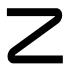
\includegraphics[keepaspectratio]{images/part001_4ea857d0.jpg}}

由例 1 可知，可能存在包含 \(\Re(\mathrm{M})\) 的子模 N，使得 M/N 的根不为零。

推论 2. —— 设 \((\mathrm{M}_{i})_{i\in\mathrm{I}}\) 是一个 A-模族，P 是它们的乘积，S 是它们的直和。我们有 \(\Re(\mathrm{P})\subset\prod_{i\in\mathrm{I}}\Re(\mathrm{M}_{i})\) 与 \(\Re(\mathrm{S})=\bigoplus_{i\in\mathrm{I}}\Re(\mathrm{M}_{i})\)。

对 \(i \in I\)，设 \(\pi_{i}\) 是从 P 到 \(M_{i}\) 的指标为 i 的投影。由命题 1，我们有 \(\pi_{i}(\mathfrak{R}(P)) \subset \mathfrak{R}(M_{i})\)（对每个 \(i \in I\)）；这就证明了第一个断言。我们有 \(S \subset P\)，因而

\[
\mathfrak {R} (S) \subset S \cap \mathfrak {R} (P) \subset S \cap \prod_ {i \in I} \mathfrak {R} (M _ {i}) = \bigoplus_ {i \in I} \mathfrak {R} (M _ {i}).
\]

此外，我们有 \(M_{i} \subset S\)，从而 \(\Re(M_{i}) \subset \Re(S)\)（对每个 \(i \in I\)），于是 \(\oplus_{i \in I} \Re(M_{i}) \subset \Re(S)\)。

存在一些模族，使得乘积的根不同构于诸根的乘积（VIII, 第 166 页，习题 3）。

命题 2. —— 设 M 是一个有限生成的 A-模。

\begin{enumerate}
\def\labelenumi{\alph{enumi})}
\item
  若 \(\mathbf{M}\) 不归结为 0，则我们有 \(\Re (\mathbf{M})\neq \mathbf{M}\)。
\item
  若 N 是 M 的一个子模，使得 \(\mathrm{N} + \Re(\mathrm{M}) = \mathrm{M}\)，则我们有 N = M。
\end{enumerate}

设 N 是 M 的一个真子模。由 VIII, 第 49 页的命题 3，存在 M 的一个包含 N 的极大子模 L。我们有 \(\mathrm{N} + \Re(\mathrm{M}) \subset \mathrm{L}\)，更必然有 \(\mathrm{N} + \Re(\mathrm{M}) \neq \mathrm{M}\)。这就证明了 b)；特例 N = 0 即给出断言 a)。

推论. —— 设 M 是一个 A-模，\((x_{i})_{i\in\mathbb{I}}\) 是 M 的一个生成族，x 是 M 的一个元素。下列性质等价：

\begin{enumerate}
\def\labelenumi{(\roman{enumi})}
\item
  我们有 \(x \in \Re(\mathbb{M})\)。
\item
  M 的每个使 \(\mathrm{N} + \mathrm{A}x = \mathrm{M}\) 的子模 N 都等于 M。
\item
  对 A 的元素的每个族 \((a_{i})_{i\in\mathrm{I}}\)，族 \((x_{i}+a_{i}x)_{i\in\mathrm{I}}\) 生成 A-模 M。
\item
  \(\Rightarrow\) (ii)：设 x 属于 \(\Re(\mathrm{M})\)。设 N 是 M 的一个子模，使得 \(N + Ax = M\)。我们有 \(N + \Re(M) = M\)；因而 A-模 M/N 等于它的根（命题 1 的推论 1, b)）。由于它是单生成的，它为零（命题 2），于是 M = N。
\item
  \(\Rightarrow\) (iii)：设 \((a_{i})_{i\in\mathrm{I}}\) 是 A 的元素的一个族。用 N 表示由族 \((x_{i}+a_{i}x)_{i\in\mathrm{I}}\) 生成的 M 的子模。我们有 \(x_{i}\in N+Ax\)（对每个 \(i\in I\)），因而 \(N+Ax=M\)。若性质 (ii) 成立，则 N 等于 M。
\item
  \(\Rightarrow\) (i)：设 x 不属于 \(\Re(\mathrm{M})\)。则存在 M 的一个不包含 x 的极大子模 N。由于 N 是极大的，我们有 \(N + Ax = M\)；因而每个元素 \(x_{i}\) 都可写成 \(y_{i} - a_{i}x\)，其中 \(y_{i} \in N\)，\(a_{i} \in A\)。族 \((x_{i} + a_{i}x)_{i \in I}\) 包含于 N，故不生成 M。
\end{enumerate}

命题 3. —— a) 半单模是无根的。

\begin{enumerate}
\def\labelenumi{\alph{enumi})}
\setcounter{enumi}{1}
\tightlist
\item
  一个模是半单的且有限生成的，当且仅当它是无根的且是阿廷的。
\end{enumerate}

按定义，单模的根归结为 0。若模 M 是半单的，则它是单子模的一个族 \((\mathrm{S}_{i})_{i\in\mathrm{I}}\) 的直和，且由上面命题 1 的推论 2，我们有 \(\mathfrak{R}(\mathrm{M})=\bigoplus_{i\in\mathrm{I}}\mathfrak{R}(\mathrm{S}_{i})\)，因而 \(\mathfrak{R}(\mathrm{M})=0\)。

此外，若 M 是有限生成的，则由 VIII, 第 71 页的命题 10，它是阿廷的。

反之，设 M 是阿廷的且无根的。把 VIII, 第 2 页应用于 M 的极大子模所成的集，存在 M 的极大子模的一个有限族 \((\mathrm{N}_{i})_{i\in\mathrm{I}}\)，其交归结为 0。于是 M 同构于 \(\bigoplus_{i\in\mathrm{I}}(\mathrm{M}/\mathrm{N}_{i})\) 的一个子模。因此，它是半单的且具有有限长度，更必然是有限生成的。

\subsection{环的根}

定义 2. —— 环 A 的雅各布森根（或简称根），记作 \(\Re(\mathrm{A})\)，是 A-模 \(A_{s}\) 的根，即 A 的极大左理想之交。

滥用语言，若我们有 \(\Re(A)=0\)，则称环 A 是无根的。

命题 4. —— 环 A 是半单的，当且仅当它是左阿廷的且无根的。

这由把命题 3, b) 应用于 A-模 \(\mathrm{A}_s\) 得出。

例. —— 1) 若 A 是一个局部环，则它有唯一的极大左理想 r，由 A 的不可逆元素组成（VIII, 第 25 页，命题 1）；于是 r 是 A 的根。特别地，体是无根的。

\pandocbounded{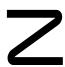
\includegraphics[keepaspectratio]{images/part001_b3b59696.jpg}}

\begin{enumerate}
\def\labelenumi{\arabic{enumi})}
\setcounter{enumi}{1}
\item
  设 K 是一个交换域，E 是形式幂级数代数 \(\mathrm{K}[[\mathrm{X}_{i}]]_{i\in\mathrm{I}}\)（变量 \(X_{i}\)、系数在 K 中）。由前一例以及 VIII, 第 26 页的例 4，E 的根由常数项为零的形式幂级数组成。注意环 E 是一个整环，且其根不归结为 0，尽管 E 是它的无根的分式域的一个子环。
\item
  设 A 是一个主理想整环，P 是由不可约元组成的一个代表系（VII, §1, No.~3, 第 3 页）。若 A 是一个体，则由例 1 它是无根的。若集 P 是无穷的，则 A 的诸极大理想 Ap 的交归结为 0，故 A 是无根的。但若 P 有限且非空，且我们令 \(x = \prod_{p \in P} p\)，则 A 的根等于 \(\cap_{p \in P} Ap = Ax\)（VII, §1, No.~2, 第 3 页，命题 4），因而不归结为 0。
\end{enumerate}

设 y 是 A 的一个非零元素；我们把它写成 \(y = up_{1}^{i_{1}} \cdots p_{r}^{i_{r}}\)，其中 u 在 A 中可逆，\(p_{1}, \ldots, p_{r}\) 是 P 中两两互异的元素，而 \(i_{1}, \ldots, i_{r}\) 是严格正的整数。环 A/Ay 的极大理想是诸理想 \(Ap_{1}/Ay, \ldots, Ap_{r}/Ay\)；因而环 A/Ay 的根是理想 \(Ap_{1} \cdots p_{r}/Ay\)。特别地，环 A/Ay 是无根的，当且仅当我们有 \(i_{1} = \cdots = i_{r} = 1\)；这时，我们称 y 是无重因子的。

命题 5. —— a) 环 A 的根是诸单 A-模的零化子之交；它也是半单 A-模的零化子中最小的一个。特别地，它是 A 的一个双边理想。若 A 不归结为 0，则 A 的根异于 A。

\begin{enumerate}
\def\labelenumi{\alph{enumi})}
\setcounter{enumi}{1}
\item
  设 \(\mathfrak{a}\) 是 A 的一个双边理想。我们有 \((\Re (\mathrm{A}) + \mathfrak{a}) / \mathfrak{a} \subset \Re (\mathrm{A} / \mathfrak{a})\)。若 \(\mathfrak{a}\) 包含于 \(\Re (\mathrm{A})\)，则我们有 \(\Re (\mathrm{A} / \mathfrak{a}) = \Re (\mathrm{A}) / \mathfrak{a}\)。
\item
  环 A/R(A) 是无根的；反之，A 的每个使 A/a 为无根的双边理想 a 都包含 R(A)。
\item
  A 的根包含于 A 的诸极大双边理想之交。
\end{enumerate}

设 \(x \in \mathrm{A}\)。说 \(x\) 属于每个单 A-模的零化子，等价于说 \(x\) 属于每个单 A-模的每个元素的零化子，换句话说（VIII, 第 46 页，命题 1），等价于属于 A 的每个极大左理想。

设 M 是一个半单 A-模。它的零化子是 M 的诸单子模的零化子之交，故它包含 \(\Re(\mathrm{A})\)。此外，若 S 是单 A-模的类所成的集（VIII, 第 51 页），则直和 \(\oplus_{\lambda\in\mathcal{S}}\lambda\) 是一个零化子为 \(\Re(\mathrm{A})\) 的半单 A-模。设 A 不归结为 0；则关系 \(\Re(\mathrm{A})\neq\mathrm{A}\) 由把 VIII, 第 153 页的命题 2, a) 应用于 A-模 \(A_{s}\) 而得。我们证明了 a)。

设 \(\mathfrak{a}\) 是 A 的一个双边理想。A/ \(\mathfrak{a}\) 的极大左理想是形如 \(\mathfrak{m}/\mathfrak{a}\) 的理想，其中 \(\mathfrak{m}\) 是 A 的包含 \(\mathfrak{a}\) 的一个极大左理想。因而环 A/ \(\mathfrak{a}\) 的根等于 A-模 \(A_s/\mathfrak{a}\) 的根。于是断言 b) 与 c) 由 VIII, 第 152 页的推论 1 得出。

设 \(\mathfrak{a}\) 是 A 的一个极大双边理想。在环 A/ \(\mathfrak{a}\) 中，仅有的双边理想是 0 与 A/ \(\mathfrak{a}\)。由于环 A/ \(\mathfrak{a}\) 不归结为 0，它的根不等于 A/ \(\mathfrak{a}\)。因而环 A/ \(\mathfrak{a}\) 是无根的，且由 c) 我们有 \(\Re(A) \subset \mathfrak{a}\)。这就证明了 d)。

我们称 A 的一个左（或右）理想是诣零理想，如果它由幂零元素组成。我们称 A 的一个双边理想 \(\mathfrak{a}\) 是幂零的，如果存在一个整数 \(n \geqslant 1\) 使得 \(\mathfrak{a}^n = 0\)，即（I, §8, No.~9, 第 107 页）使得我们有 \(x_1 \cdots x_n = 0\)，只要 \((x_1, \ldots, x_n)\) 是 \(\mathfrak{a}\) 中元素的一个序列。每个幂零双边理想都是诣零理想，但可能存在不包含于任何幂零双边理想之中的诣零理想（VIII, 第 167 页，习题 9）。

定理 1（雅各布森）. —— 环 A 的根由这样的元素 \(x \in \mathbf{A}\) 组成：\(1 + ax\) 对每个 \(a \in \mathbf{A}\) 都是左可逆的（I, §2, No.~3, 第 15 页）。它也是最大的双边理想 \(\mathfrak{a}\)：\(1 + x\) 对每个 \(x \in \mathfrak{a}\) 都可逆。\(\mathbf{A}\) 的根包含 \(\mathbf{A}\) 的每个左诣零理想。

元素 1 生成 A-模 \(A_{s}\)，且 \(1 + ax\) 左可逆当且仅当它生成 A-模 \(A_{s}\)。因而定理 1 的第一个断言是命题 2 的推论（VIII, 第 153 页）的一个特例。

设 \(x \in \Re(\mathrm{A})\)。由上述，\(1 + x\) 左可逆；设 \(y\) 是 \(\mathrm{A}\) 中使 \(y(1 + x) = 1\) 的一个元素。于是我们有 \(1 - y = yx\)，故 \(1 - y\) 属于 \(\Re(\mathrm{A})\)；因而 \(y\) 左可逆。由于 \(y\) 也右可逆，它可逆（I, §2, No.~3, 第 16 页，命题 3），而它的右逆 \(1 + x\) 也可逆。

设 a 是 A 的一个左理想，使得 \(1 + x\) 对每个 \(x \in a\) 都可逆。例如当 a 是诣零理想时即属此情形，因为关系 \(x^{n} = 0\) 蕴含 \(1 - x + \cdots + (-x)^{n-1}\) 是 \(1 + x\) 的逆。设 \(x \in a\)。对每个 \(a \in A\)，我们有 \(ax \in a\)，故 \(1 + ax\) 可逆；因而我们有 \(x \in \Re(A)\)。于是 a 包含于 \(\Re(A)\)。

推论 1. —— A 的根等于反环 A° 的根，即 A 的极大右理想之交。

对每个 \(x \in \Re(A)\)，\(1 + x\) 在环 A 中可逆，因而在环 \(A^{\circ}\) 中可逆。由于 \(\Re(A)\) 是 \(A^{\circ}\) 的一个双边理想，我们有 \(\Re(A) \subset \Re(A^{\circ})\)。交换 A 与 \(A^{\circ}\) 的角色即得等式。

推论 2. —— A 的一个元素可逆，当且仅当它在环 A/ \(\Re(A)\) 中的典范像可逆。

该条件显然是必要的。我们来证明它是充分的。设 x 是 A 的一个元素，它在环 \(\mathrm{A}/\Re(\mathrm{A})\) 中的典范像可逆。则存在 A 的一个元素 y，使得 xy 属于 \(1 + \Re(\mathrm{A})\)。由定理 1，xy 可逆；因而 x 右可逆。x 左可逆的证明是类似的。

推论 3. —— 一族环 \((\mathrm{A}_{i})_{i\in\mathrm{I}}\) 的乘积的根是诸 \(\mathfrak{R}(\mathrm{A}_{i})\) 的乘积。

设 \(x = (x_{i})_{i\in \mathrm{I}}\) 是 \(\prod_{i\in \mathrm{I}}\mathrm{A}_{i}\) 的一个元素。对每个元素 \(a = (a_{i})_{i\in \mathrm{I}}\)（\(\prod_{i\in \mathrm{I}}\mathrm{A}_{i}\) 的），元素 \(1 + ax\) 左可逆当且仅当 \(1 + a_{i}x_{i}\) 在 \(\mathrm{A}_i\) 中左可逆（对每个 \(i\in \mathrm{I}\)）。由此即得推论 3。

推论 4. —— 环 A 是局部的，当且仅当环 A/ \(\Re(A)\) 是一个体。若属此情形，则 \(\Re(A)\) 是 A 的不可逆元素所成的集。

用 r 表示 A 的不可逆元素所成的集。若环 A 是局部的，则它的根等于 r（VIII, 第 154 页，例 1），且环 A/r 是一个体（VIII, 第 26 页）。反之，设环 A/R(A) 是一个体。由推论 2，我们有 \(\mathfrak{r} = \Re(\mathrm{A})\)，故 r 是 A 的一个双边理想。由此推得环 A 是局部的（VIII, 第 26 页，定义 1）。

例. —— 4) 设 K 是一个整环，I 是一个非空集，A 是多项式环 \(K[X_{i}]_{i\in I}\)。我们来证明环 A 是无根的。A 中仅有的可逆元素是 K 的可逆元素（IV, §1, No.~5, 第 9 页，推论 2）。设 \(f \in \Re(A)\)。选取一个元素 \(i \in I\)。则 \(1 + fX_{i}\) 可逆（定理 1），这蕴含 f = 0。

\pandocbounded{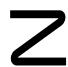
\includegraphics[keepaspectratio]{images/part001_fdd5464e.jpg}}

注意当 K 是一个交换域时，环 \(A = K[X_{i}]_{i \in I}\) 是 \(B = K[[X_{i}]]_{i \in I}\) 的一个子环，且我们有 \(\Re(A) = 0\) 与 \(A \cap \Re(B) \neq 0\)（参见 VIII, 第 154 页，例 2）。

\begin{enumerate}
\def\labelenumi{\arabic{enumi})}
\setcounter{enumi}{4}
\tightlist
\item
  设 \(\mathfrak{a}\) 是 A 的一个双边理想。A 上的 \(\mathfrak{a}\)-进拓扑是与 A 的环结构相容、且使诸理想 \(\mathfrak{a}^n\)（对 \(n \geqslant 1\)）构成 0 的一个基本邻域系的那个拓扑（《一般拓扑》，III, §6, No.~3, 第 275 页，例 3）。设环 A 对此拓扑是豪斯多夫的且完备的（《一般拓扑》，III, §6, No.~5, 第 276 页）；例如当理想 \(\mathfrak{a}\) 幂零时即属此情形。于是对每个 \(x \in \mathfrak{a}\)，级数 \(\sum_{n=0}^{\infty} (-x)^n\) 收敛。设 \(y\) 是它的和。我们有 \(y - 1 = \sum_{n=1}^{\infty} (-x)^n = -xy\)，因而 \((1 + x)y = 1\)。同样，我们有 \(y(1 + x) = 1\)，故 \(1 + x\) 可逆。由定理 1，由此推得理想 \(\mathfrak{a}\) 包含于 A 的根中。
\end{enumerate}

注. —— 1) 由定理 1，环 A 的每个左诣零理想都包含于它的根中。设 x 是 A 的一个幂零的中心元素；则 Ax 是 A 的一个诣零理想，故 x 属于 A 的根。然而，可能存在 A 的非零幂零元素，而 A 却是无根的。例如，对每个整数 \(n \geqslant 2\)，体 K 上的矩阵环 \(\mathbf{M}_{n}(\mathrm{K})\) 是单的，因而是无根的（VIII, 第 154 页，命题 4），而它含有幂零元素，例如矩阵单位 \(E_{ij}\)（\(i \neq j\)）。

\pandocbounded{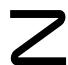
\includegraphics[keepaspectratio]{images/part001_653588be.jpg}}

\begin{enumerate}
\def\labelenumi{\arabic{enumi})}
\setcounter{enumi}{1}
\tightlist
\item
  设 A 是一个交换环。A 的幂零元素 \(a\) 所成的集是 A 的一个理想 \(\mathfrak{N}(\mathrm{A})\)，称为 A 的幂零根；它是 A 的诸素理想之交（V, §15, No.~1, 第 118 页，命题 2）。我们有 \(\mathfrak{N}(A) \subset \mathfrak{R}(A)\)；*当 A 是一个阿廷环（VIII, 第 173 页，推论 2）或是交换域上的一个有限生成交换代数（《交换代数》，V, §3, n°4, 定理 3）时，我们有等式*。我们当然可能有 \(\mathfrak{N}(A) \neq \mathfrak{R}(A)\)。当 A 是环 K{[}{[}X{]}{]}（其中 K 是一个交换域）时即属此情形：这时我们有 \(\mathfrak{N}(A) = 0\) 与 \(\mathfrak{R}(A) = AX\)（VIII, 第 154 页，例 2）。
\end{enumerate}

\subsection{中山引理}

命题 6. —— 对每个 A-模 M，我们有 \(\Re(A)M \subset \Re(M)\)。若 A-模 M 是投射的，则有等式。

设 P 是 M 的一个极大子模；A-模 M/P 是单的，故由 VIII, 第 155 页的命题 5，它被 \(\Re(\mathrm{A})\) 零化。于是对 M 的每个极大子模 P，我们有 \(\Re(\mathrm{A})\mathrm{M}\subset\mathrm{P}\)，因而 \(\Re(\mathrm{A})\mathrm{M}\subset\Re(\mathrm{M})\)。

我们显然有 \(\mathfrak{R}(A_{s})=\mathfrak{R}(A)A_{s}\)。若 A-模 M 是投射的，则存在一个 A-模 N，使得 \(M\oplus N\) 是自由的，即是模的一个族 \((\mathrm{L}_{i})_{i\in\mathrm{I}}\)（同构于 \(A_{s}\)）的直和。由 VIII, 第 152 页的推论 2，我们有 \(\mathfrak{R}(M\oplus N)=\mathfrak{R}(M)\oplus\mathfrak{R}(N)\) 与 \(\mathfrak{R}\big(\bigoplus_{i\in I}L_{i}\big)=\bigoplus_{i\in I}\mathfrak{R}(L_{i})\)。于是，\(\mathfrak{R}(M)=\mathfrak{R}(A)M\) 由等式 \(\mathfrak{R}(L_{i})=\mathfrak{R}(A)L_{i}\) 推出。

定理 2（``中山引理''）. —— 设 M 是一个 A-模，a 是 A 的一个双边理想。设下列条件之一满足：

\begin{enumerate}
\def\labelenumi{(\roman{enumi})}
\item
  A-模 M 是有限生成的，且 \(\mathfrak{a}\) 包含于 A 的根中。
\item
  理想 \(\mathfrak{a}\) 是幂零的。
\end{enumerate}

若 N 是 M 的一个子模，使得 \(M = N + aM\)，则我们有 N = M。特别地，若模 M 非零，则我们有 \(M \neq aM\)。

设 M 是有限生成的，且我们有 \(\mathfrak{a} \subset \Re(\mathrm{A})\)。设 N 是 M 的一个子模，使得 \(M = N + aM\)。由命题 6，我们有 \(M = N + \Re(M)\)，故由 VIII, 第 153 页的命题 2, b) 得 M = N。

现在设 a 是幂零的，并设 N 是 M 的一个子模，使得 \(M = N + aM\)。对整数 \(n \geqslant 0\) 作归纳，我们建立关系 \(M = N + a^{n}M\)。按假设，存在一个整数 \(n \geqslant 0\) 使得 \(a^{n} = 0\)；因而 M = N。

定理的最后一个断言由上述取 N 为 0 即得。

推论 1. —— 我们保持定理 2 的假设。设 \((x_{i})_{i\in\mathrm{I}}\) 是 M 的元素的一个族，\(\overline{x}_{i}\) 是 \(x_{i}\) 在 M/aM 中的典范像。若族 \((\overline{x}_{i})_{i\in\mathrm{I}}\) 生成 (A/a)-模 M/aM，则族 \((x_{i})_{i\in\mathrm{I}}\) 生成 A-模 M。

这由把定理 2 应用于由族 \((x_{i})_{i\in \mathbf{I}}\) 生成的 M 的子模 N 得出。

推论 2. —— 我们保持定理 2 的假设。此外，设 M' 是一个 A-模，u : M' → M 是一个同态。若由 u 通过取商得到的从 M'/aM' 到 M/aM 的同态 \(\overline{u}\) 是满射，则 u 是满射。

只需把定理 2 应用于 u 的像 N：事实上，\(\overline{u}\) 的像是 \((\mathrm{N} + \mathfrak{aM})/\mathfrak{aM}\)，故 \(\overline{u}\) 是满射当且仅当我们有 \(N + aM = M\)。

\subsection{幂等元的提升}

引理 1. —— 设 a 是环 A 中一个使 \(a - a^{2}\) 幂零的元素。存在 \(\mathrm{X} + (\mathrm{X} - \mathrm{X}^{2})\mathbf{Z}[\mathrm{X}]\) 中的一个多项式 P，使得 \(\mathrm{P}(a)\) 在 A 中是幂等的。

设 n 是一个使 \((a - a^{2})^{n} = 0\) 的严格正整数。令 \(\mathrm{P}(\mathrm{X}) = 1 - (1 - \mathrm{X}^{n})^{n}\)。多项式 \(\mathrm{P}(\mathrm{X})\) 是 \(X^{n}\) 的倍式，多项式 \(1 - \mathrm{P}(\mathrm{X})\) 是 \((1 - \mathrm{X})^{n}\) 的倍式，故 \(\mathrm{P}(\mathrm{X}) - \mathrm{P}(\mathrm{X})^{2}\) 是 \((\mathrm{X} - \mathrm{X}^{2})^{n}\) 的倍式，且我们有 \(\mathrm{P}(a) = \mathrm{P}(a)^{2}\)。此外，\(\mathrm{X} - \mathrm{P}(\mathrm{X})\) 同时是 X 与 1 - X 的倍式，因而是 \(X - X^{2}\) 的倍式。

命题 7. —— 设 a 是 A 的一个双边诣零理想，\(\overline{e}\) 是环 A/a 中的一个幂等元。存在 A 中的一个幂等元 e，它在 A/a 中的典范像等于 \(\overline{e}\)。

设 \(a\) 是 \(\overline{e}\) 在 \(\mathbf{A}\) 中的任意一个代表。元素 \(a - a^2\)（\(\mathbf{A}\) 的）是幂零的，因为它属于 \(\mathfrak{a}\)。选取一个满足引理 1 的条件的多项式 \(\mathrm{P} \in \mathbf{Z}[\mathrm{X}]\)。我们有 \(a - \mathrm{P}(a) \in \mathrm{A}(a - a^2)\)，故元素 \(e = \mathrm{P}(a)\)（\(\mathbf{A}\) 的）具有所要的性质。

\pandocbounded{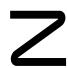
\includegraphics[keepaspectratio]{images/part001_2ad691f6.jpg}}

设 \(\bar{e}\) 属于环 A/a 的中心。不一定存在 A 的中心 Z 中提升 \(\bar{e}\) 的幂等元 e（VIII, 第 172 页，习题 31）。然而，若 \(\bar{e}\) 属于 Z 在 A/a 中的像，则它可提升为 Z 中的一个幂等元，因为 \(Z \cap a\) 是 Z 的一个诣零理想。

推论 1. —— 设 M 与 P 是 A-模，u 是从 P 到 M 的一个满 A-线性映射。设 P 是投射的，且存在 A 的一个幂零双边理想 \(\mathfrak{a}\)，使得 \(u\) 的核 N 包含于 \(\mathfrak{aP}\)。设 \(\mathrm{M}'\) 与 \(\mathrm{M}''\) 是 M 的子模，其直和为 M。则 P 是子模 \(\mathrm{P}'\) 与 \(\mathrm{P}''\) 的直和，使得 \(u(\mathrm{P}') = \mathrm{M}'\) 且 \(u(\mathrm{P}''') = \mathrm{M}''\)。

用 B 表示 \(\operatorname{End}_{\mathrm{A}}(\mathrm{P})\) 中由满足 \(f(\mathrm{N}) \subset \mathrm{N}\) 的 P 的自同态 f 组成的子环。设 \(\overline{B}\) 是 M 的自同态环。对 \(f \in B\)，设 \(\overline{f}\) 是满足 \(\overline{f} \circ u = u \circ f\) 的 M 的唯一自同态。映射 \(f \mapsto \overline{f}\) 是从 B 到 \(\overline{B}\) 的一个环同态。由于模 P 是投射的，这个同态是满射；其核 b 由自同态 \(f \in B\)（满足 \(f(\mathrm{P}) \subset \mathrm{N}\)）组成。设 n 是一个使 \(a^{n} = 0\) 的自然数。我们有

\[
\mathrm{P} = \mathfrak {a} ^ {0} \mathrm{P} \supset \mathfrak {a} ^ {1} \mathrm{P} \supset \dots \supset \mathfrak {a} ^ {n - 1} \mathrm{P} \supset \mathfrak {a} ^ {n} \mathrm{P} = 0,
\]

且对每个 \(f \in b\) 与每个整数 \(j \geqslant 0\)，

\[
f (\mathfrak {a} ^ {j} \mathrm{P}) = \mathfrak {a} ^ {j} f (\mathrm{P}) \subset \mathfrak {a} ^ {j} \mathrm{N} \subset \mathfrak {a} ^ {j + 1} \mathrm{P}
\]

因为按假设 \(N \subset aP\)。于是我们有 \(f(P) \subset a^{j}P\)（对每个自然数 j 及每个 \(f \in b^{j}\)）。特别地，我们有 \(b^{n} = 0\)。

设 \(\varepsilon'\) 是 M 的以 M' 为像、以 M'\,` 为核的投影算子。由把命题 7 应用于环 B 与幂零双边理想 b，存在 B 中的一个幂等元 \(e'\)，使得 \(\overline{e'} = \varepsilon'\)，即 \(\varepsilon' \circ u = u \circ e'\)。令 \(e'' = 1 - e'\)，\(\varepsilon'' = \overline{e''}\)，P' = \(e'(P)\)，P'\,' = \(e''(P)\)。则 P 是子模 P' 与 P'\,' 的直和，且我们有

\[
u (\mathrm{P} ^ {\prime}) = u (e ^ {\prime} (\mathrm{P})) = \varepsilon^ {\prime} (u (\mathrm{P})) = \varepsilon^ {\prime} (\mathrm{M}) = \mathrm{M} ^ {\prime};
\]

等式 \(u(\mathrm{P}'') = \mathrm{M}''\) 的证明是类似的。

推论 2. —— 设 A 是一个环，a 是 A 的一个幂零双边理想。若 P 是一个投射 A-模，则 P/aP 是 A/a 上的一个投射模，且 A-模 P 是不可分解的当且仅当 A/a-模 P/aP 是不可分解的。

设 P 是一个投射 A-模，\(\overline{P}\) 是 A/a-模 P/aP。A-模 P 为零当且仅当 \(\overline{P}\) 为零（VIII, 第 158 页，定理 2）。现在设 \(P \neq 0\)。由于 A/a-模 \(\overline{P}\) 同构于 \(\overline{A} \otimes_{A} P\)，它是投射的（II, §5, No.~1, 第 279 页，命题 4 的推论）。若 P 是不可分解的，则由推论 1，\(\overline{P}\) 也是不可分解的。反之，设 P 是可分解的且非零，并设 \(P'\) 与 \(P''\) 是 P 的两个非零子模，使得 \(P = P' \oplus P''\)。由中山引理（VIII, 第 158 页，定理 2），我们有 \(P' + aP \neq P\) 与 \(P'' + aP \neq P\)；若 \(\overline{P}'\) 与 \(\overline{P}''\) 是 \(P'\) 与 \(P''\) 在 \(\overline{P}\) 中的典范像，则我们有 \(\overline{P}' \neq \overline{P}\)，\(\overline{P}'' \neq \overline{P}\)，以及 \(\overline{P} = \overline{P}' \oplus \overline{P}''\)。这就证明 \(\overline{P}\) 是可分解的。
